\documentclass[a4paper,10pt]{article}

% --- PACKAGES ---
\usepackage[utf8]{inputenc}
\usepackage[T1]{fontenc}
\usepackage[margin=0.75in]{geometry}
\usepackage{graphicx}
\usepackage{amsmath, amssymb}
\usepackage{booktabs}
\usepackage{float}
\usepackage{hyperref}
\usepackage{listings}
\usepackage{xcolor}
\usepackage{subcaption}
\usepackage{enumitem}
\usepackage{caption}

% --- HYPERLINK STYLE ---
\hypersetup{
    colorlinks=true,
    linkcolor=blue,
    urlcolor=blue,
    citecolor=blue
}

% --- COMPACT LAYOUT ---
\captionsetup{font=small,skip=2pt}
\setlist{nosep,leftmargin=*}
\setlength{\parindent}{0pt}
\setlength{\parskip}{2pt}
\setlength{\textfloatsep}{4pt}
\setlength{\floatsep}{4pt}
\setlength{\intextsep}{4pt}
\linespread{0.95}

% --- CODE LISTING STYLE ---
\definecolor{codegreen}{rgb}{0,0.6,0}
\definecolor{codegray}{rgb}{0.5,0.5,0.5}
\definecolor{codepurple}{rgb}{0.58,0,0.82}
\definecolor{backcolour}{rgb}{0.96,0.96,0.96}

\lstdefinestyle{pystyle}{
    backgroundcolor=\color{backcolour},
    commentstyle=\color{codegreen},
    keywordstyle=\color{magenta},
    stringstyle=\color{codepurple},
    basicstyle=\ttfamily\scriptsize,
    breaklines=true,
    captionpos=b,
    numbers=none,
    showstringspaces=false,
    tabsize=2
}
\lstset{style=pystyle}

% --- SIMPLE HORIZONTAL RULE ---
\newcommand{\hr}{\rule{\linewidth}{0.5pt}}

\begin{document}

% ============================================================
% COVER PAGE
% ============================================================
\begin{titlepage}
\thispagestyle{empty}
\centering

% ---------- UNIVERSITY / INSTITUTION HEADER ----------
\vspace*{0.4cm}
{\large\scshape United International University}\\[0.15cm]
{\small Department of Computer Science \& Engineering}\\[0.35cm]

\rule{\linewidth}{1pt}\\[0.05cm]
\rule{\linewidth}{0.4pt}

\vspace{1.4cm}

% ---------- COURSE ----------
{\large\bfseries CSE 4889}\\[0.25cm]
{\Large\bfseries Machine Learning Laboratory}\\[0.9cm]

% ---------- REPORT TITLE ----------
{\Huge\bfseries Assignment Report}\\[0.5cm]
{\large\itshape Implementation and Evaluation of Learning Algorithms}\\[0.35cm]

% ---------- ALGORITHM CATEGORIES ----------
{\small
Clustering \(\cdot\) Density-Based \(\cdot\) Semi-Supervised \(\cdot\) Ensemble \(\cdot\)
Neural \(\cdot\) Probabilistic \(\cdot\) Margin-Based \(\cdot\)
Foundation-Model \(\cdot\) Non-Parametric
}\\[0.5cm]

\rule{\linewidth}{0.4pt}
\rule{\linewidth}{1pt}

\vspace{1.6cm}

% ---------- COURSE INFORMATION ----------
\begin{minipage}{0.85\textwidth}
\centering
\begin{tabular}{@{}p{5cm}p{7cm}@{}}
\toprule
\textbf{Course Teacher} & Dr.\ Ohidujjaman \\
\textbf{Department}     & Computer Science \& Engineering \\
\textbf{Institution}    & United International University \\
\textbf{Language}       & Python 3.x \\
\textbf{Platform}       & Jupyter Notebook (Google Colab) \\
\textbf{Global Seed}    & 42 \\
\bottomrule
\end{tabular}
\end{minipage}

\vspace{1.8cm}

% ---------- SUBMITTED BY ----------
{\large\bfseries Submitted By}\\[0.4cm]
\begin{tabular}{@{}ll@{}}
\toprule
\textbf{Name} & \textbf{Student ID} \\
\midrule
Fariya Nika Oshru              & 0112330006 \\
Md.\ Akib Mehedi               & 0112330681 \\
Md.\ Toufiq Imroz Khealid Khan & 0112330984 \\
\bottomrule
\end{tabular}

\vfill

% ---------- DATE ----------
{\small \today}\\[0.4cm]

\end{titlepage}

% ============================================================
% TABLE OF CONTENTS
% ============================================================
\tableofcontents
\newpage

% ============================================================
% CLUSTERING
% ============================================================
\section{Clustering}

% ------------------------------------------------------------
% EXPERIMENT 1: K-MEANS CLUSTERING
% ------------------------------------------------------------
\subsection{Experiment 1: K-Means Clustering}

\subsubsection{Objective}
Implement K-Means to partition data into \(K\) clusters, find centroids, visualize clusters, and evaluate using Inertia and Silhouette Score.

\subsubsection{Dataset}
Synthetic blobs from \texttt{make\_blobs()}: 300 samples, 3 centers, 2 features, std \(=1.0\), random state \(=42\).

\subsubsection{Theory}
K-Means is unsupervised. It minimizes within-cluster sum of squares (WCSS):
\[
J = \sum_{j=1}^{K} \sum_{x_i \in C_j} \| x_i - \mu_j \|^2
\]
where \(\mu_j\) is the centroid of cluster \(C_j\). Distance uses Euclidean metric. Centroids update as the mean of assigned points. Inertia is the WCSS value; Silhouette Score measures cluster separation (\(-1\) to \(1\), higher is better).

\subsubsection{Procedure}
\begin{enumerate}[nosep]
    \item Import libraries.
    \item Generate dataset.
    \item Set \(K=3\), fit K-Means (\texttt{n\_init=10}, \texttt{random\_state=42}).
    \item Predict labels, get centroids.
    \item Plot clusters and centroids.
    \item Compute Inertia and Silhouette Score.
\end{enumerate}

\subsubsection{Code}
\begin{lstlisting}[language=Python, caption={K-Means Implementation}]
import numpy as np
import matplotlib.pyplot as plt
from sklearn.datasets import make_blobs
from sklearn.cluster import KMeans
from sklearn.metrics import silhouette_score

X, y = make_blobs(n_samples=300, centers=3, cluster_std=1.0, random_state=42)

k = 3
kmeans = KMeans(n_clusters=k, random_state=42, n_init=10)
labels = kmeans.fit_predict(X)
centroids = kmeans.cluster_centers_

plt.figure(figsize=(8,5))
plt.scatter(X[:,0], X[:,1], c=labels, cmap='viridis', s=50)
plt.scatter(centroids[:,0], centroids[:,1], marker='X', s=200, color='red', label='Centroids')
plt.title('K-Means Clustering')
plt.xlabel('Feature 1'); plt.ylabel('Feature 2'); plt.legend()
plt.show()

inertia = kmeans.inertia_
silhouette = silhouette_score(X, labels)
print("Inertia:", inertia)
print("Silhouette Score:", silhouette)
for i in range(k):
    print(f"Cluster {i}: {np.sum(labels == i)} points")
\end{lstlisting}

\subsubsection{Results}
\begin{table}[H]
\centering
\caption{K-Means Metrics}
\begin{tabular}{ll}
\toprule
\textbf{Metric} & \textbf{Value} \\
\midrule
Number of Clusters (\(K\)) & 3 \\
Inertia & 566.86 \\
Silhouette Score & 0.8480 \\
\bottomrule
\end{tabular}
\end{table}

\begin{figure}[H]
\centering
\begin{subfigure}{0.48\textwidth}
    \centering
    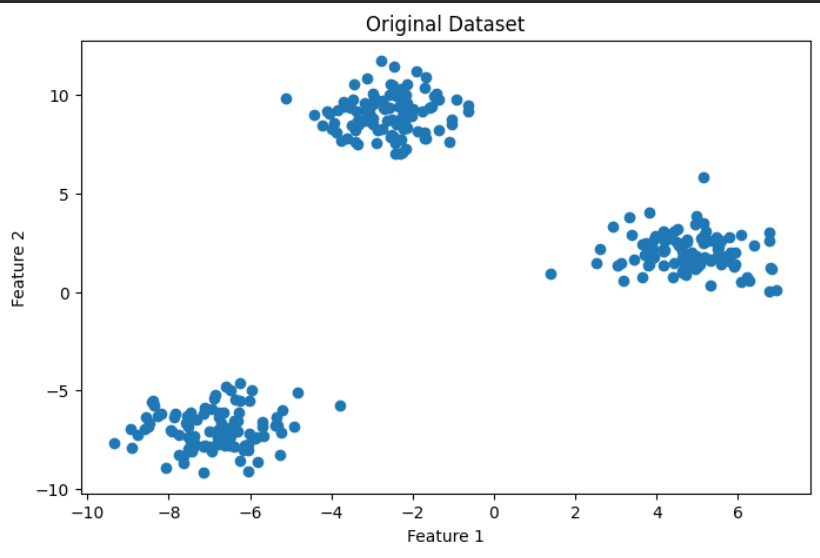
\includegraphics[width=\linewidth]{km_dataset.png}
    \caption{Original dataset}
\end{subfigure}
\hfill
\begin{subfigure}{0.48\textwidth}
    \centering
    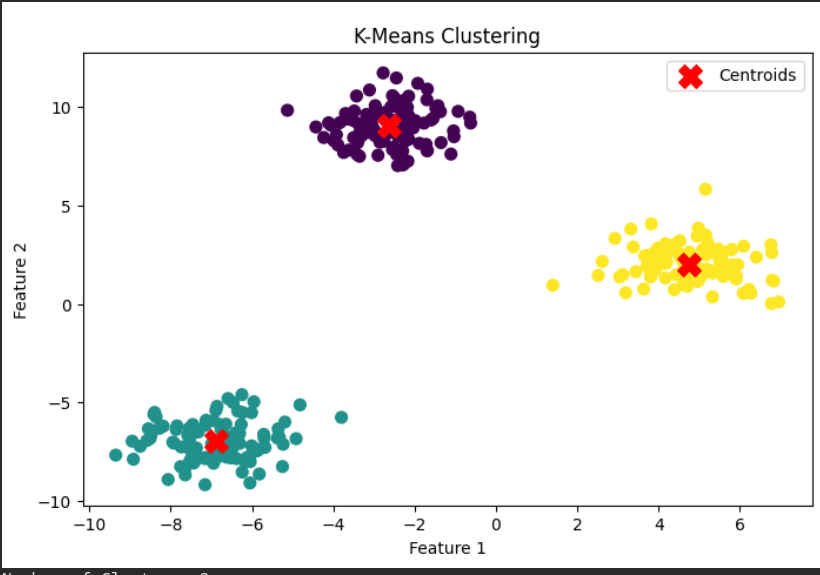
\includegraphics[width=\linewidth]{km_output.png}
    \caption{K-Means result with centroids}
\end{subfigure}
\caption{K-Means clustering on synthetic blobs.}
\end{figure}

\subsubsection{Discussion \& Conclusion}
K-Means successfully partitioned the data into three well-separated clusters (Silhouette \(=0.848\)). Inertia \(=566.86\) indicates compact clusters. The algorithm is simple and fast but requires \(K\) beforehand, is sensitive to initialization, and assumes spherical clusters of similar size. Using \texttt{n\_init=10} mitigates poor local minima.

% ------------------------------------------------------------
% EXPERIMENT 2: MODIFIED K-MEANS
% ------------------------------------------------------------
\subsection{Experiment 2: Modified K-Means Clustering}

\subsubsection{Objective}
Implement Modified K-Means using maximum-distance-based centroid initialization, and compare with standard K-Means.

\subsubsection{Dataset}
Same synthetic blobs: 300 samples, 3 centers, 2 features, std \(=1.0\), random state \(=42\).

\subsubsection{Theory}
Standard K-Means uses random initialization, which can lead to poor local minima. Modified K-Means picks initial centroids far apart:
\begin{enumerate}[nosep]
    \item Pick first centroid (e.g., \(X_0\)).
    \item For each point, compute its minimum distance to selected centroids.
    \item Pick the point with the largest minimum distance as the next centroid.
    \item Repeat until \(K\) centroids are chosen.
\end{enumerate}
Then standard K-Means runs with these fixed starting centroids.

\subsubsection{Procedure}
\begin{enumerate}[nosep]
    \item Generate dataset.
    \item Select \(K=3\) initial centroids via maximum-distance rule.
    \item Fit K-Means with \texttt{init=initial\_centroids}, \texttt{n\_init=1}.
    \item Plot clusters and final centroids.
    \item Compute Inertia and Silhouette Score.
\end{enumerate}

\subsubsection{Code}
\begin{lstlisting}[language=Python, caption={Modified K-Means Implementation}]
import numpy as np
import matplotlib.pyplot as plt
from sklearn.datasets import make_blobs
from sklearn.cluster import KMeans
from sklearn.metrics import silhouette_score

X, y = make_blobs(n_samples=300, centers=3, cluster_std=1.0, random_state=42)

def modified_initialization(X, k):
    centroids = [X[0]]
    for _ in range(1, k):
        distances = np.array([min(np.linalg.norm(x - c) for c in centroids) for x in X])
        centroids.append(X[np.argmax(distances)])
    return np.array(centroids)

k = 3
initial_centroids = modified_initialization(X, k)
print("Initial Centroids:\n", initial_centroids)

kmeans = KMeans(n_clusters=k, init=initial_centroids, n_init=1, random_state=42)
labels = kmeans.fit_predict(X)
centroids = kmeans.cluster_centers_

plt.figure(figsize=(8,5))
plt.scatter(X[:,0], X[:,1], c=labels, cmap='viridis', s=50)
plt.scatter(centroids[:,0], centroids[:,1], marker='X', s=200, color='red', label='Centroids')
plt.title('Modified K-Means Clustering')
plt.xlabel('Feature 1'); plt.ylabel('Feature 2'); plt.legend()
plt.show()

print("Inertia:", kmeans.inertia_)
print("Silhouette Score:", silhouette_score(X, labels))
for i in range(k):
    print(f"Cluster {i}: {np.sum(labels == i)} points")
\end{lstlisting}

\subsubsection{Results}
\begin{table}[H]
\centering
\caption{Modified K-Means Metrics}
\begin{tabular}{ll}
\toprule
\textbf{Metric} & \textbf{Value} \\
\midrule
Number of Clusters (\(K\)) & 3 \\
Initialization & Maximum-Distance-Based \\
Inertia & 566.86 \\
Silhouette Score & 0.8480 \\
\bottomrule
\end{tabular}
\end{table}

\begin{figure}[H]
\centering
\begin{subfigure}{0.48\textwidth}
    \centering
    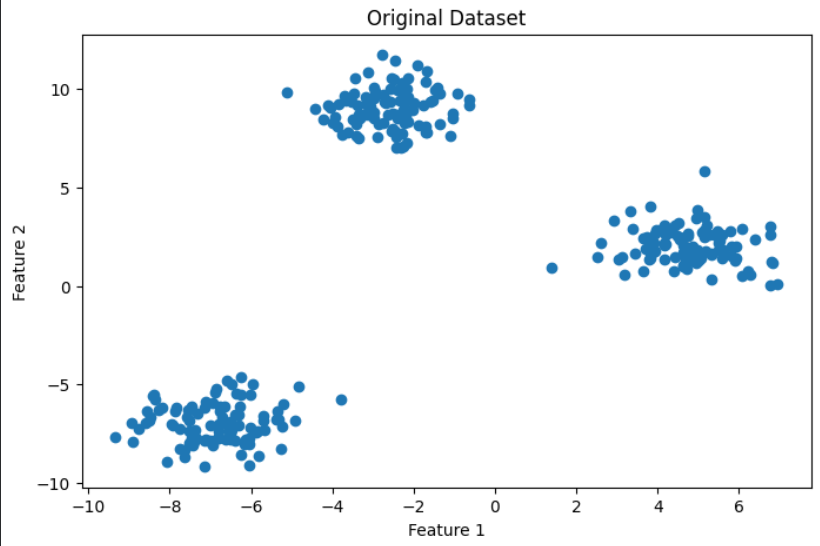
\includegraphics[width=\linewidth]{mkm_dataset.png}
    \caption{Original dataset}
\end{subfigure}
\hfill
\begin{subfigure}{0.48\textwidth}
    \centering
    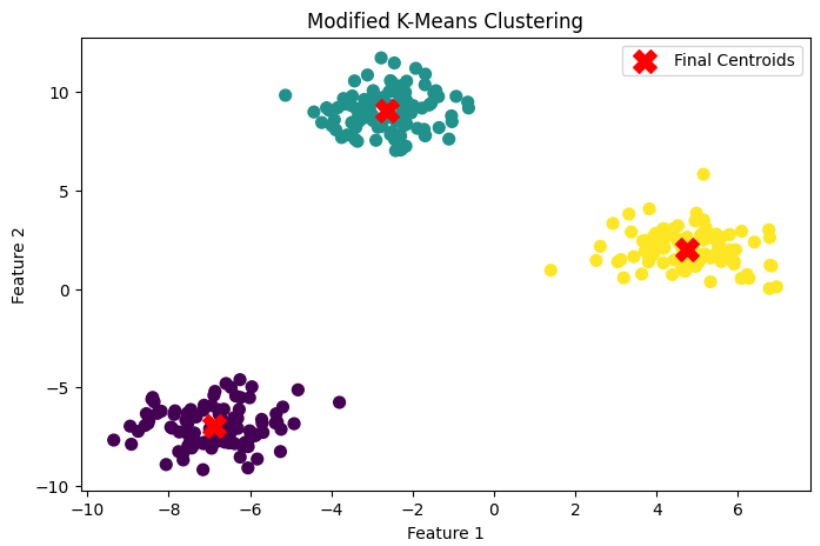
\includegraphics[width=\linewidth]{mkm_output.png}
    \caption{Modified K-Means result}
\end{subfigure}
\caption{Modified K-Means with maximum-distance initialization.}
\end{figure}

\subsubsection{Discussion \& Conclusion}
The maximum-distance rule gave well-separated initial centroids, producing the same clustering quality as standard K-Means (Silhouette \(=0.848\), Inertia \(=566.86\)). The method provides a more controlled starting point and reduces reliance on random initialization. Limitations remain: \(K\) must be preset, outliers can be picked as centroids, and clusters are still assumed compact and spherical.
% ------------------------------------------------------------
% EXPERIMENT 3: HIERARCHICAL CLUSTERING
% ------------------------------------------------------------
\subsection{Experiment 3: Hierarchical Clustering}

\subsubsection{Objective}
Implement Agglomerative Hierarchical Clustering, visualize a dendrogram, and evaluate using Silhouette Score.

\subsubsection{Dataset}
Synthetic blobs: 100 samples, 3 centers, 2 features, std \(=1.0\), random state \(=42\).

\subsubsection{Theory}
Hierarchical Clustering groups points into a hierarchy. No \(K\) needed upfront; it is chosen by cutting the dendrogram.

\textbf{Types:} Agglomerative (bottom-up, used here) and Divisive (top-down).

\textbf{Linkage:} Single (min), Complete (max), Average, Ward (minimum variance increase).

\textbf{Dendrogram:} Tree showing merge distances.

\textbf{Silhouette Score:} Measures separation (\(-1\) to \(1\), higher is better).

\subsubsection{Procedure}
\begin{enumerate}[nosep]
    \item Generate dataset.
    \item Compute Ward linkage and plot dendrogram.
    \item Set \(K=3\), fit Agglomerative Clustering.
    \item Plot clusters and compute Silhouette Score.
\end{enumerate}

\subsubsection{Code}
\begin{lstlisting}[language=Python, caption={Hierarchical Clustering Implementation}]
import numpy as np
import matplotlib.pyplot as plt
from sklearn.datasets import make_blobs
from sklearn.cluster import AgglomerativeClustering
from sklearn.metrics import silhouette_score
from scipy.cluster.hierarchy import dendrogram, linkage

X, y = make_blobs(n_samples=100, centers=3, cluster_std=1.0, random_state=42)

Z = linkage(X, method='ward')
plt.figure(figsize=(12,6))
dendrogram(Z, truncate_mode='lastp', p=30)
plt.title('Hierarchical Clustering Dendrogram')
plt.xlabel('Data Points / Clusters'); plt.ylabel('Euclidean Distance')
plt.show()

k = 3
hc = AgglomerativeClustering(n_clusters=k, linkage='ward')
labels = hc.fit_predict(X)

plt.figure(figsize=(8,5))
plt.scatter(X[:,0], X[:,1], c=labels, cmap='viridis', s=50)
plt.title('Agglomerative Hierarchical Clustering')
plt.xlabel('Feature 1'); plt.ylabel('Feature 2')
plt.show()

print("Silhouette Score:", silhouette_score(X, labels))
for i in range(k):
    print(f"Cluster {i}: {np.sum(labels == i)} points")
\end{lstlisting}

\subsubsection{Results}
\begin{table}[H]
\centering
\caption{Hierarchical Clustering Metrics}
\begin{tabular}{ll}
\toprule
\textbf{Metric} & \textbf{Value} \\
\midrule
Number of Clusters (\(K\)) & 3 \\
Linkage & Ward \\
Distance Metric & Euclidean \\
Silhouette Score & 0.8470 \\
\bottomrule
\end{tabular}
\end{table}

\begin{figure}[H]
\centering
\begin{subfigure}{0.48\textwidth}
    \centering
    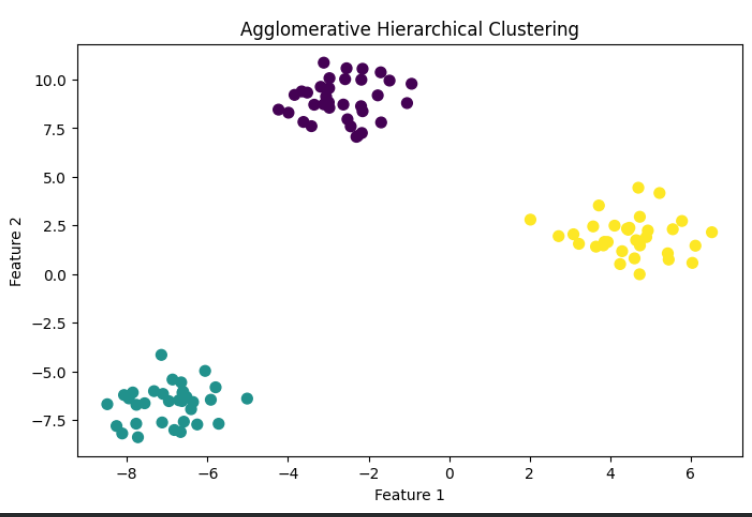
\includegraphics[width=\linewidth]{hc_output.png}
    \caption{Agglomerative clustering result}
\end{subfigure}
\hfill
\begin{subfigure}{0.48\textwidth}
    \centering
    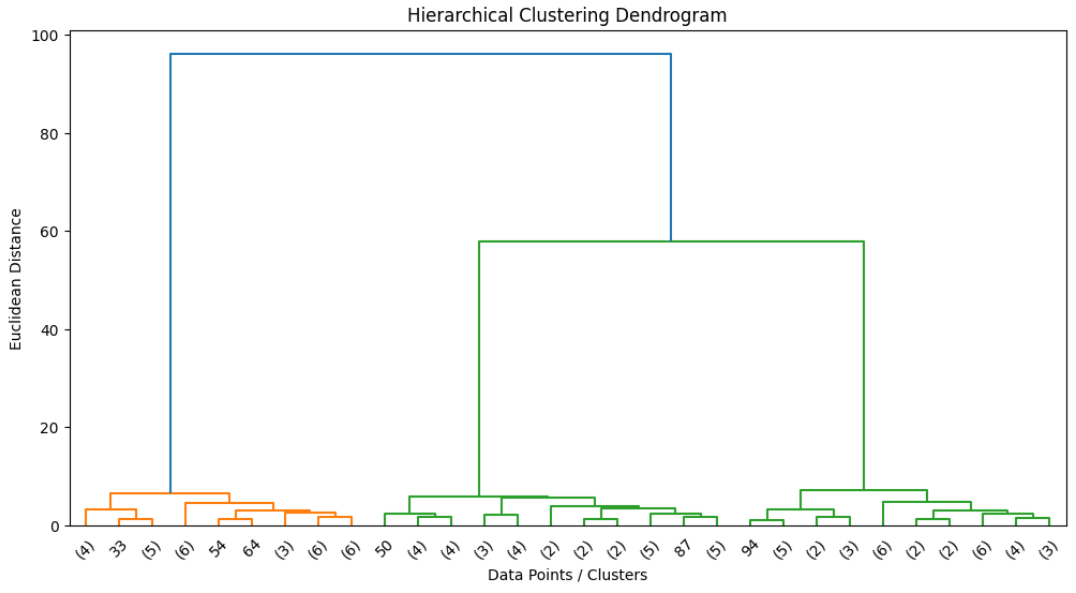
\includegraphics[width=\linewidth]{hc_dendrogram.png}
    \caption{Dendrogram (Ward linkage)}
\end{subfigure}
\caption{Hierarchical clustering on synthetic blobs.}
\end{figure}

\subsubsection{Discussion \& Conclusion}
Agglomerative Clustering with Ward linkage produced three balanced clusters (34/33/33) with Silhouette \(=0.847\), indicating well-separated groups. The dendrogram visually confirms natural grouping at \(K=3\). Limitations: computationally heavy for large datasets, sensitive to linkage/distance choice, merges are irreversible, and outliers can distort results.

% ------------------------------------------------------------
% EXPERIMENT 4: FUZZY C-MEANS CLUSTERING
% ------------------------------------------------------------
\subsection{Experiment 4: Fuzzy C-Means Clustering}

\subsubsection{Objective}
Implement Fuzzy C-Means (FCM) to assign soft memberships, compute cluster centers, and evaluate with Silhouette Score.

\subsubsection{Dataset}
Synthetic blobs: 300 samples, 3 centers, 2 features, std \(=1.0\), random state \(=42\).

\subsubsection{Theory}
FCM allows each point to belong to multiple clusters with membership values summing to 1:
\[
\sum_{j=1}^{C} u_{ij} = 1
\]
Cluster centers:
\[
v_j = \frac{\sum_{i=1}^{N} u_{ij}^{m} x_i}{\sum_{i=1}^{N} u_{ij}^{m}}
\]
Objective:
\[
J_m = \sum_{i=1}^{N} \sum_{j=1}^{C} u_{ij}^{m} \| x_i - v_j \|^2
\]
Fuzziness \(m\) controls softness (\(m=2\) typical). Hard labels are taken as \(\arg\max_j u_{ij}\).

\textbf{vs.\ K-Means:} K-Means is hard (single cluster per point); FCM is soft (multi-cluster membership).

\subsubsection{Procedure}
\begin{enumerate}[nosep]
    \item Install/import \texttt{scikit-fuzzy}.
    \item Generate dataset.
    \item Set \(C=3\), \(m=2.0\); fit FCM on \(X^T\).
    \item Convert memberships to hard labels.
    \item Plot clusters and centers; compute Silhouette Score.
\end{enumerate}

\subsubsection{Code}
\begin{lstlisting}[language=Python, caption={Fuzzy C-Means Implementation}]
!pip install scikit-fuzzy

import numpy as np
import matplotlib.pyplot as plt
import skfuzzy as fuzz
from sklearn.datasets import make_blobs
from sklearn.metrics import silhouette_score

X, y = make_blobs(n_samples=300, centers=3, cluster_std=1.0, random_state=42)

c, m = 3, 2.0
data = X.T

centers, membership, *_ , fpc, iterations = fuzz.cluster.cmeans(
    data, c=c, m=m, error=0.005, maxiter=1000, init=None, seed=42)

labels = np.argmax(membership, axis=0)

plt.figure(figsize=(8,5))
plt.scatter(X[:,0], X[:,1], c=labels, cmap='viridis', s=50)
plt.scatter(centers[:,0], centers[:,1], marker='X', s=200, color='red', label='Centers')
plt.title('Fuzzy C-Means Clustering')
plt.xlabel('Feature 1'); plt.ylabel('Feature 2'); plt.legend()
plt.show()

print("Silhouette Score:", silhouette_score(X, labels))
print("FPC:", fpc, "| Iterations:", iterations)
for i in range(c):
    print(f"Cluster {i}: {np.sum(labels == i)} points")
\end{lstlisting}

\subsubsection{Results}
\begin{table}[H]
\centering
\caption{Fuzzy C-Means Metrics}
\begin{tabular}{ll}
\toprule
\textbf{Metric} & \textbf{Value} \\
\midrule
Number of Clusters (\(C\)) & 3 \\
Fuzziness (\(m\)) & 2.0 \\
Silhouette Score & \textit{(fill in)} \\
Fuzzy Partition Coefficient (FPC) & \textit{(fill in)} \\
Iterations & \textit{(fill in)} \\
\bottomrule
\end{tabular}
\end{table}

\begin{figure}[H]
\centering
\begin{subfigure}{0.48\textwidth}
    \centering
    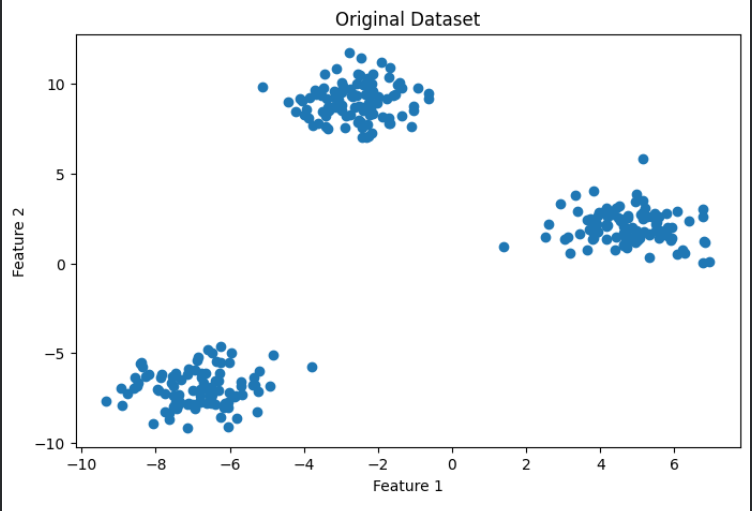
\includegraphics[width=\linewidth]{fcm_dataset.png}
    \caption{Original dataset}
\end{subfigure}
\hfill
\begin{subfigure}{0.48\textwidth}
    \centering
    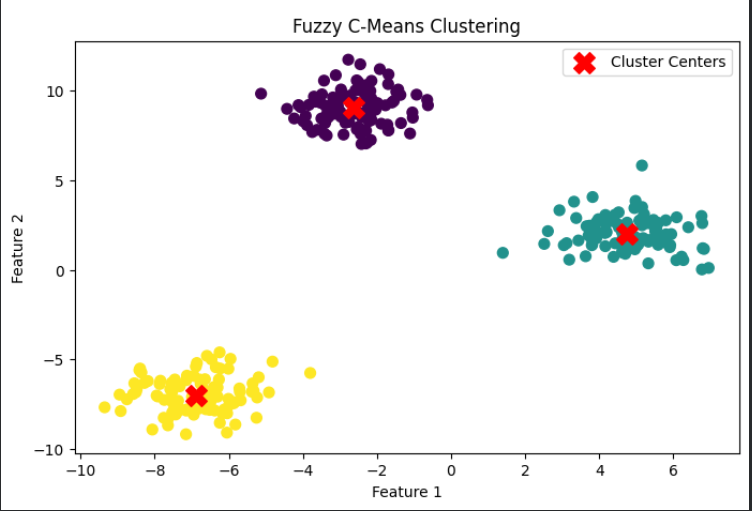
\includegraphics[width=\linewidth]{fcm_output.png}
    \caption{FCM result with centers}
\end{subfigure}
\caption{Fuzzy C-Means on synthetic blobs.}
\end{figure}

\subsubsection{Discussion \& Conclusion}
FCM assigned soft memberships (summing to 1) instead of hard labels, allowing overlap handling. Points near cluster centers had high membership for one cluster; boundary points had more balanced values. Hard labels were obtained via \(\arg\max\). FPC measured partition clarity; Silhouette measured separation. FCM is more flexible than K-Means for overlapping clusters, but requires \(C\) in advance, is sensitive to \(m\), initialization, and outliers, and is costlier on large data.




% ============================================================
% DENSITY-BASED LEARNING
% ============================================================
\section{Density-Based Learning}
% Insert experiments here (e.g., DBSCAN, OPTICS, Mean Shift).
% ------------------------------------------------------------
% EXPERIMENT 5: DBSCAN CLUSTERING
% ------------------------------------------------------------
\subsection{Experiment 5: DBSCAN Clustering}

\subsubsection{Objective}
Implement DBSCAN to find density-based clusters, detect noise, and evaluate with Silhouette Score.

\subsubsection{Dataset}
Synthetic moons: 300 samples, noise \(=0.08\), 2 features, random state \(=42\).

\subsubsection{Theory}
DBSCAN groups points by density. No \(K\) needed. Parameters:
\begin{itemize}[nosep]
    \item \texttt{eps}: neighborhood radius.
    \item \texttt{min\_samples}: minimum neighbors for a core point.
\end{itemize}
Point types: core, border, noise (label \(-1\)). Steps: pick point, find neighbors, expand cluster if core, mark noise otherwise. Silhouette is computed on non-noise points.

\subsubsection{Procedure}
\begin{enumerate}[nosep]
    \item Generate moons dataset.
    \item Set \texttt{eps=0.2}, \texttt{min\_samples=5}, fit DBSCAN.
    \item Plot clusters and noise.
    \item Compute Silhouette Score (excluding noise).
\end{enumerate}

\subsubsection{Code}
\begin{lstlisting}[language=Python, caption={DBSCAN Implementation}]
import numpy as np
import matplotlib.pyplot as plt
from sklearn.datasets import make_moons
from sklearn.cluster import DBSCAN
from sklearn.metrics import silhouette_score

X, y = make_moons(n_samples=300, noise=0.08, random_state=42)

db = DBSCAN(eps=0.2, min_samples=5)
labels = db.fit_predict(X)

plt.figure(figsize=(8,5))
plt.scatter(X[:,0], X[:,1], c=labels, cmap='viridis', s=50)
plt.title('DBSCAN Clustering')
plt.xlabel('Feature 1'); plt.ylabel('Feature 2')
plt.colorbar(label='Cluster Label')
plt.show()

n_clusters = len(set(labels)) - (1 if -1 in labels else 0)
n_noise = np.sum(labels == -1)
mask = labels != -1

print("Clusters:", n_clusters, "| Noise:", n_noise)
if n_clusters >= 2 and np.sum(mask) > n_clusters:
    print("Silhouette Score:", silhouette_score(X[mask], labels[mask]))
for i in sorted(set(labels)):
    print(f"Label {i}: {np.sum(labels == i)} points")
\end{lstlisting}

\subsubsection{Results}
\begin{table}[H]
\centering
\caption{DBSCAN Metrics}
\begin{tabular}{ll}
\toprule
\textbf{Metric} & \textbf{Value} \\
\midrule
Epsilon (\texttt{eps}) & 0.2 \\
Minimum Samples & 5 \\
Number of Clusters & 2 \\
Number of Noise Points & 0 \\
Silhouette Score & 0.3273 \\
\bottomrule
\end{tabular}
\end{table}

\begin{figure}[H]
\centering
\begin{subfigure}{0.48\textwidth}
    \centering
    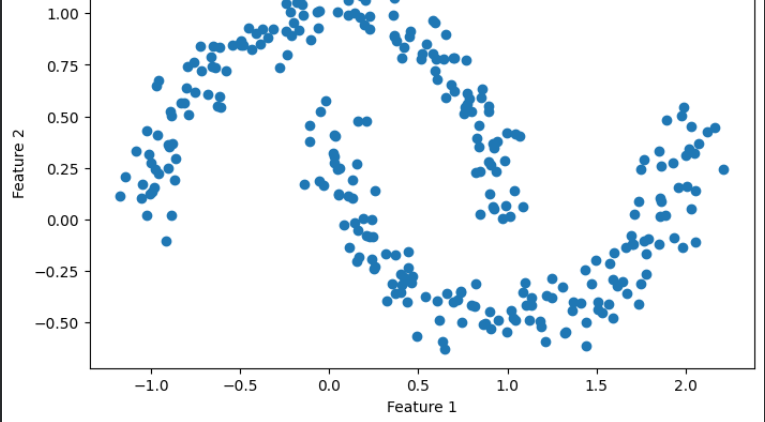
\includegraphics[width=\linewidth]{dbscan_dataset.png}
    \caption{Original moons}
\end{subfigure}
\hfill
\begin{subfigure}{0.48\textwidth}
    \centering
    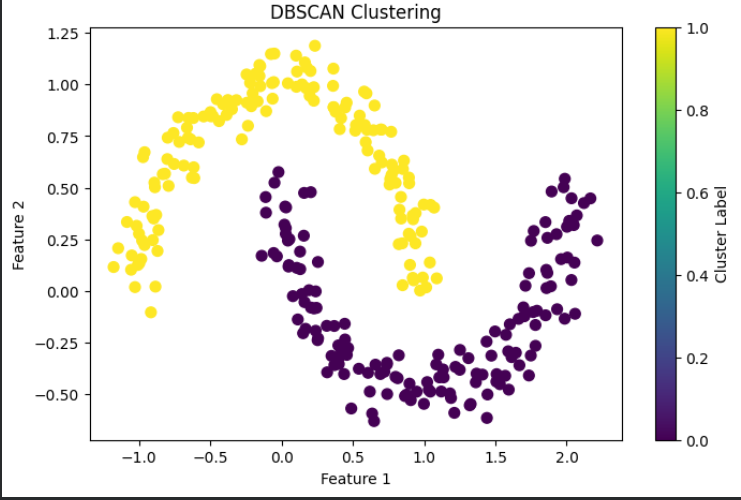
\includegraphics[width=\linewidth]{dbscan_output.png}
    \caption{DBSCAN result}
\end{subfigure}
\caption{DBSCAN on two-moon dataset.}
\end{figure}

\subsubsection{Discussion \& Conclusion}
DBSCAN correctly identified the two non-spherical moon clusters with zero noise points. The moderate Silhouette Score (\(0.3273\)) reflects the curved shape, which standard distance-based metrics penalize. DBSCAN is robust to outliers and needs no \(K\), but results depend heavily on \texttt{eps} and \texttt{min\_samples}, and performance drops with varying densities or high dimensions.

% ------------------------------------------------------------
% EXPERIMENT 6: HDBSCAN CLUSTERING
% ------------------------------------------------------------
\subsection{Experiment 6: HDBSCAN Clustering}

\subsubsection{Objective}
Implement HDBSCAN to cluster variable-density data without a fixed epsilon and evaluate with Silhouette Score.

\subsubsection{Dataset}
Synthetic blobs: 300 samples, 3 centers, 2 features, std \(=[0.5, 1.0, 1.5]\), random state \(=42\).

\subsubsection{Theory}
HDBSCAN extends DBSCAN by building a hierarchy of clusters across multiple density levels. No \texttt{eps} is needed.

\textbf{Parameters:} \texttt{min\_cluster\_size} (minimum points per cluster), \texttt{min\_samples} (density strictness), \texttt{metric} (Euclidean here).

\textbf{Steps:} compute core distances \(\rightarrow\) mutual reachability distance
\[
d_{mr}(a,b) = \max(core_k(a),\, core_k(b),\, d(a,b))
\]
build minimum spanning tree \(\rightarrow\) hierarchy \(\rightarrow\) extract stable clusters \(\rightarrow\) mark noise.

\textbf{vs.\ DBSCAN:} handles varying densities, no fixed epsilon, but is more complex.

\subsubsection{Procedure}
\begin{enumerate}[nosep]
    \item Install/import \texttt{hdbscan}.
    \item Generate variable-density dataset.
    \item Fit HDBSCAN (\texttt{min\_cluster\_size=10}, \texttt{min\_samples=5}).
    \item Plot clusters; compute Silhouette (excluding noise).
    \item Print probabilities for the first 10 points.
\end{enumerate}

\subsubsection{Code}
\begin{lstlisting}[language=Python, caption={HDBSCAN Implementation}]
!pip install hdbscan

import numpy as np
import matplotlib.pyplot as plt
import hdbscan
from sklearn.datasets import make_blobs
from sklearn.metrics import silhouette_score

X, y = make_blobs(n_samples=300, centers=3,
                  cluster_std=[0.5, 1.0, 1.5], random_state=42)

clusterer = hdbscan.HDBSCAN(min_cluster_size=10, min_samples=5, metric='euclidean')
labels = clusterer.fit_predict(X)

plt.figure(figsize=(8,5))
plt.scatter(X[:,0], X[:,1], c=labels, cmap='viridis', s=50)
plt.title('HDBSCAN Clustering')
plt.xlabel('Feature 1'); plt.ylabel('Feature 2')
plt.colorbar(label='Cluster Label')
plt.show()

mask = labels != -1
n_clusters = len(set(labels)) - (1 if -1 in labels else 0)
n_noise = np.sum(labels == -1)

print("Clusters:", n_clusters, "| Noise:", n_noise)
if n_clusters >= 2 and np.sum(mask) > n_clusters:
    print("Silhouette Score:", silhouette_score(X[mask], labels[mask]))
print("Probabilities (first 10):", clusterer.probabilities_[:10])
\end{lstlisting}

\subsubsection{Results}
\begin{table}[H]
\centering
\caption{HDBSCAN Metrics}
\begin{tabular}{ll}
\toprule
\textbf{Metric} & \textbf{Value} \\
\midrule
Minimum Cluster Size & 10 \\
Minimum Samples & 5 \\
Number of Clusters & 3 \\
Number of Noise Points & 0 \\
Silhouette Score & 0.8541 \\
\bottomrule
\end{tabular}
\end{table}

\begin{figure}[H]
\centering
\begin{subfigure}{0.48\textwidth}
    \centering
    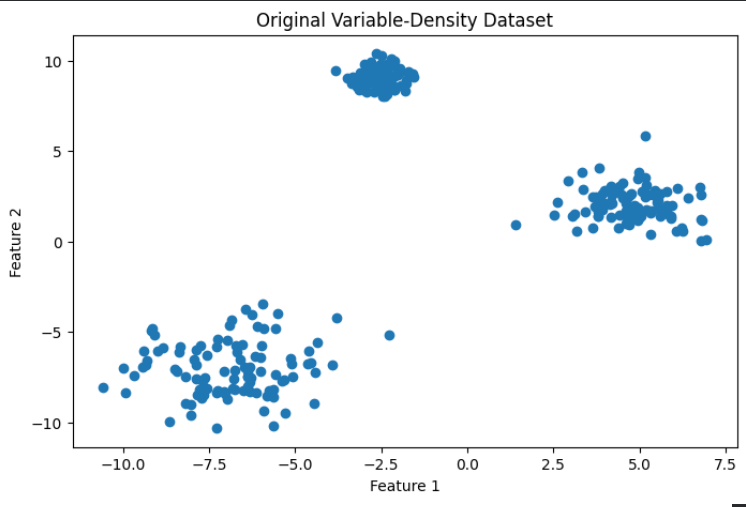
\includegraphics[width=\linewidth]{hdbscan_dataset.png}
    \caption{Original variable-density data}
\end{subfigure}
\hfill
\begin{subfigure}{0.48\textwidth}
    \centering
    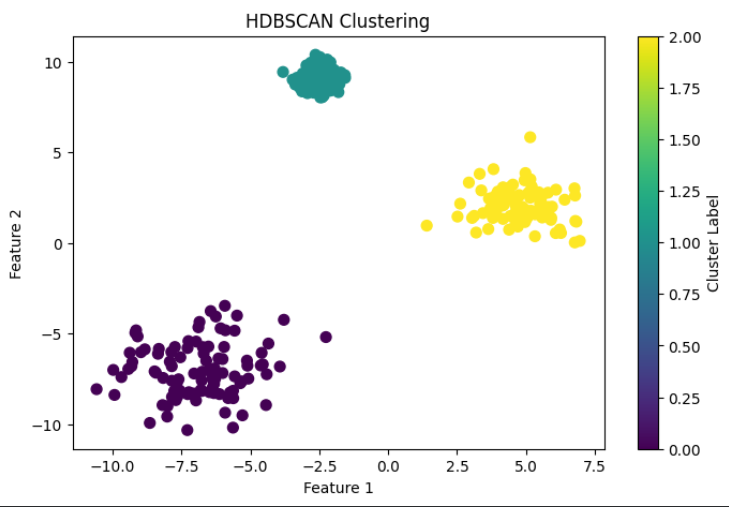
\includegraphics[width=\linewidth]{hdbscan_output.png}
    \caption{HDBSCAN result}
\end{subfigure}
\caption{HDBSCAN on variable-density synthetic blobs.}
\end{figure}

\subsubsection{Discussion \& Conclusion}
HDBSCAN recovered all three variable-density clusters with no noise and a strong Silhouette Score (\(0.8541\)). Membership probabilities showed confident assignments for dense-core points (probability \(=1\)) and lower values near boundaries. HDBSCAN is more flexible than DBSCAN for varying densities, but is computationally heavier and sensitive to \texttt{min\_cluster\_size} and \texttt{min\_samples}.


% ============================================================
% SEMI-SUPERVISED LEARNING
% ============================================================
\section{Semi-Supervised Learning}
% ------------------------------------------------------------
% EXPERIMENT 7: SELF-TRAINING (SEMI-SUPERVISED)
% ------------------------------------------------------------
\subsection{Experiment 7: Self-Training for Semi-Supervised Learning}

\subsubsection{Objective}
Implement Self-Training with an SVM base classifier using 20\% labeled and 80\% unlabeled training data, and evaluate with Accuracy and Classification Report.

\subsubsection{Dataset}
Breast Cancer Wisconsin: 569 samples, 30 features, 2 classes (malignant, benign). Train/test split 80/20; of the training set, 20\% labeled and 80\% unlabeled.

\subsubsection{Theory}
Semi-Supervised Learning uses both labeled and unlabeled data. Self-Training iteratively:
\begin{enumerate}[nosep]
    \item Train base model on labeled data.
    \item Predict pseudo-labels for unlabeled data.
    \item Add high-confidence predictions (above threshold) to training set.
    \item Retrain and repeat until convergence.
\end{enumerate}
Key parameters: \texttt{threshold} (confidence, here \(0.8\)), \texttt{max\_iter} (\(10\)). Base model: SVM with \texttt{probability=True}.

\subsubsection{Procedure}
\begin{enumerate}[nosep]
    \item Load dataset, split, scale features.
    \item Mark 20\% of training labels; set rest to \(-1\).
    \item Fit \texttt{SelfTrainingClassifier} with SVM.
    \item Predict on test set; compute Accuracy and Classification Report.
    \item Report pseudo-labeled count and iterations.
\end{enumerate}

\subsubsection{Code}
\begin{lstlisting}[language=Python, caption={Self-Training Implementation}]
import numpy as np
from sklearn.datasets import load_breast_cancer
from sklearn.model_selection import train_test_split
from sklearn.preprocessing import StandardScaler
from sklearn.semi_supervised import SelfTrainingClassifier
from sklearn.svm import SVC
from sklearn.metrics import accuracy_score, classification_report

data = load_breast_cancer()
X, y = data.data, data.target

X_train, X_test, y_train, y_test = train_test_split(
    X, y, test_size=0.2, random_state=42, stratify=y)

scaler = StandardScaler()
X_train = scaler.fit_transform(X_train)
X_test = scaler.transform(X_test)

indices = np.arange(len(X_train))
labeled_idx, unlabeled_idx = train_test_split(
    indices, test_size=0.8, random_state=42, stratify=y_train)

y_semi = np.full(len(y_train), -1)
y_semi[labeled_idx] = y_train[labeled_idx]

base_model = SVC(probability=True, random_state=42)
self_training = SelfTrainingClassifier(
    estimator=base_model, threshold=0.8, max_iter=10, verbose=True)

self_training.fit(X_train, y_semi)
y_pred = self_training.predict(X_test)

print("Accuracy:", accuracy_score(y_test, y_pred))
print(classification_report(y_test, y_pred, target_names=data.target_names))

pseudo = np.sum(self_training.transduction_[unlabeled_idx] != -1)
print("Pseudo-Labeled:", pseudo, "| Final Labeled:",
      np.sum(self_training.transduction_ != -1),
      "| Iterations:", self_training.n_iter_)
\end{lstlisting}

\subsubsection{Results}
\begin{table}[H]
\centering
\caption{Self-Training Setup \& Results}
\begin{tabular}{ll}
\toprule
\textbf{Item} & \textbf{Value} \\
\midrule
Base Estimator & SVM (RBF, \texttt{probability=True}) \\
Confidence Threshold & 0.8 \\
Max Iterations & 10 \\
Total Training Samples & 455 \\
Initial Labeled Samples & 91 \\
Initial Unlabeled Samples & 364 \\
Pseudo-Labeled Samples & 349 \\
Final Labeled Samples & 440 \\
Iterations Run & 6 \\
Accuracy & 0.9737 \\
\bottomrule
\end{tabular}
\end{table}

\begin{figure}[H]
    \centering
    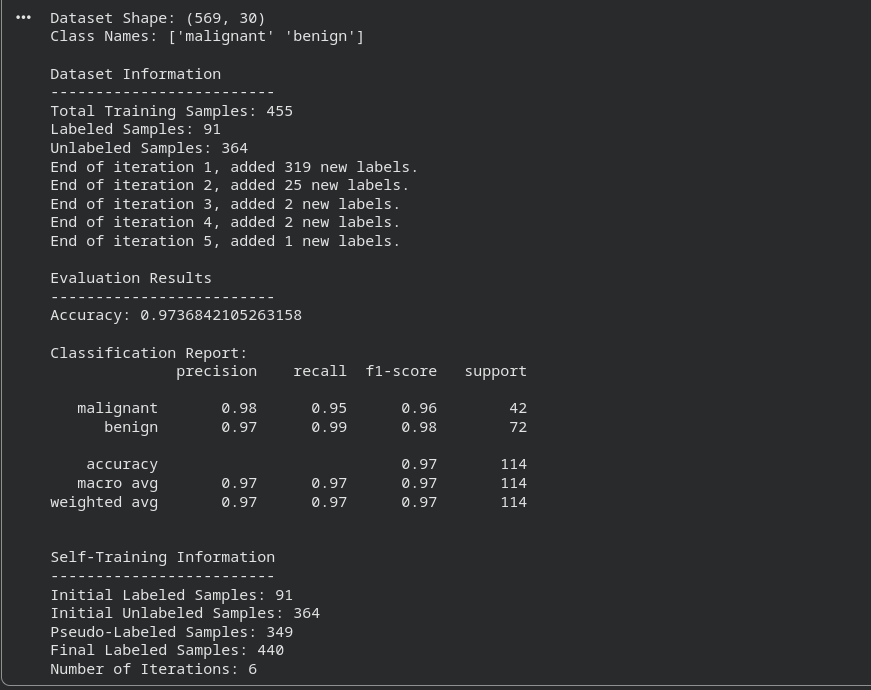
\includegraphics[width=0.85\linewidth]{selftrain_output.png}
    \caption{Self-training output: metrics and pseudo-label info.}
\end{figure}

\subsubsection{Discussion \& Conclusion}
Self-Training achieved \(97.37\%\) accuracy on the test set. Starting from only 91 labeled samples, the model pseudo-labeled 349 of 364 unlabeled samples over 6 iterations, reaching 440 final labeled samples. Precision/recall/F1 were \(\approx 0.97\) for both classes. The method effectively exploits unlabeled data but is sensitive to the confidence threshold and initial model quality; incorrect pseudo-labels can propagate.
% ============================================================
% ENSEMBLE LEARNING
% ============================================================
\section{Ensemble Learning}
% ------------------------------------------------------------
% EXPERIMENT 8: RANDOM FOREST REGRESSION
% ------------------------------------------------------------
\subsection{Experiment 8: Random Forest Regression (RFR)}

\subsubsection{Objective}
Implement Random Forest Regression to predict continuous values and evaluate with MAE, MSE, RMSE, and R\(^2\).

\subsubsection{Dataset}
California Housing: 20{,}640 samples, 8 features, target \(=\) median house value.

\subsubsection{Theory}
RFR is an ensemble of decision trees. Each tree trains on a bootstrap sample with random feature subsets; the final prediction is the average across trees. This reduces overfitting and handles non-linear relationships.

\textbf{Parameters:} \texttt{n\_estimators} (number of trees), \texttt{max\_depth}, \texttt{random\_state}.

\textbf{Metrics:} MAE, MSE, RMSE (lower is better); R\(^2\) (closer to 1 is better).

\subsubsection{Procedure}
\begin{enumerate}[nosep]
    \item Load dataset, split 80/20.
    \item Fit \texttt{RandomForestRegressor(n\_estimators=100)}.
    \item Predict on test set.
    \item Compute MAE, MSE, RMSE, R\(^2\).
    \item Plot actual vs.\ predicted.
\end{enumerate}

\subsubsection{Code}
\begin{lstlisting}[language=Python, caption={Random Forest Regression Implementation}]
import numpy as np
import pandas as pd
import matplotlib.pyplot as plt
from sklearn.datasets import fetch_california_housing
from sklearn.model_selection import train_test_split
from sklearn.ensemble import RandomForestRegressor
from sklearn.metrics import mean_absolute_error, mean_squared_error, r2_score

data = fetch_california_housing()
X, y = data.data, data.target

X_train, X_test, y_train, y_test = train_test_split(
    X, y, test_size=0.2, random_state=42)

model = RandomForestRegressor(n_estimators=100, random_state=42, n_jobs=-1)
model.fit(X_train, y_train)
y_pred = model.predict(X_test)

mae  = mean_absolute_error(y_test, y_pred)
mse  = mean_squared_error(y_test, y_pred)
rmse = np.sqrt(mse)
r2   = r2_score(y_test, y_pred)

print("MAE:", mae, "| MSE:", mse)
print("RMSE:", rmse, "| R2:", r2)

plt.figure(figsize=(8,6))
plt.scatter(y_test, y_pred, alpha=0.5)
plt.plot([y_test.min(), y_test.max()],
         [y_test.min(), y_test.max()], 'r--')
plt.xlabel('Actual'); plt.ylabel('Predicted')
plt.title('Random Forest Regression: Actual vs Predicted')
plt.show()
\end{lstlisting}

\subsubsection{Results}
\begin{table}[H]
\centering
\caption{RFR Setup \& Metrics}
\begin{tabular}{ll}
\toprule
\textbf{Item} & \textbf{Value} \\
\midrule
\texttt{n\_estimators} & 100 \\
Test Size & 0.2 \\
Random State & 42 \\
MAE & 0.3275 \\
MSE & 0.2554 \\
RMSE & 0.5053 \\
R\(^2\) Score & 0.8051 \\
\bottomrule
\end{tabular}
\end{table}

\begin{figure}[H]
    \centering
    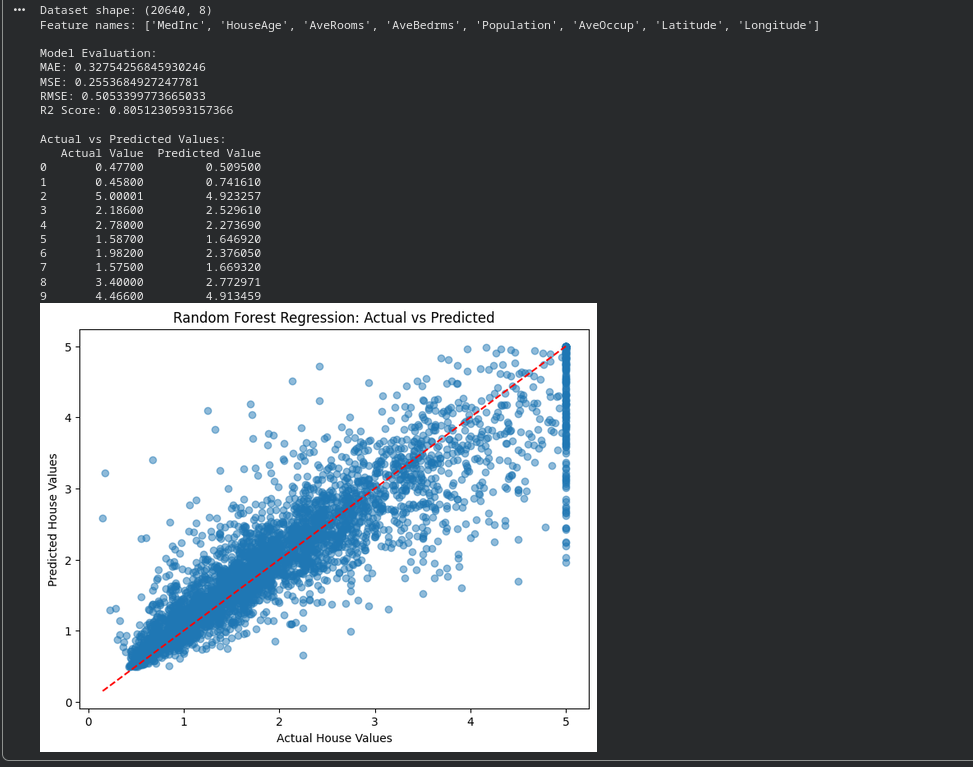
\includegraphics[width=0.7\linewidth]{rfr_output.png}
    \caption{RFR actual vs.\ predicted house values.}
\end{figure}

\subsubsection{Discussion \& Conclusion}
RFR achieved R\(^2=0.8051\), RMSE \(=0.5053\), and MAE \(=0.3275\), indicating strong predictive performance on the California Housing dataset. The scatter plot shows points clustered near the reference line, with larger deviations at extreme house values. Limitations: slower training with many trees, needs parameter tuning, and performance depends on feature quality.

% ------------------------------------------------------------
% EXPERIMENT 9: RANDOM FOREST CLASSIFICATION
% ------------------------------------------------------------
\subsection{Experiment 9: Random Forest Classification (RFC)}

\subsubsection{Objective}
Implement Random Forest Classification to predict class labels and evaluate with Accuracy, Precision, Recall, F1, and Confusion Matrix.

\subsubsection{Dataset}
Breast Cancer Wisconsin: 569 samples, 30 features, 2 classes (malignant, benign).

\subsubsection{Theory}
RFC is an ensemble of decision trees. Each tree trains on a bootstrap sample with random feature subsets; the final label is decided by majority voting. Reduces overfitting and provides feature importance.

\textbf{Parameters:} \texttt{n\_estimators}, \texttt{max\_depth}, \texttt{random\_state}.

\textbf{Metrics:} Accuracy, Precision, Recall, F1-score, Confusion Matrix.

\subsubsection{Procedure}
\begin{enumerate}[nosep]
    \item Load dataset, split 80/20 (stratified).
    \item Fit \texttt{RandomForestClassifier(n\_estimators=100)}.
    \item Predict on test set.
    \item Compute metrics, confusion matrix, and top-10 feature importances.
\end{enumerate}

\subsubsection{Code}
\begin{lstlisting}[language=Python, caption={Random Forest Classification Implementation}]
import numpy as np
import pandas as pd
import matplotlib.pyplot as plt
from sklearn.datasets import load_breast_cancer
from sklearn.model_selection import train_test_split
from sklearn.ensemble import RandomForestClassifier
from sklearn.metrics import (accuracy_score, classification_report,
                             confusion_matrix, ConfusionMatrixDisplay)

data = load_breast_cancer()
X, y = data.data, data.target

X_train, X_test, y_train, y_test = train_test_split(
    X, y, test_size=0.2, random_state=42, stratify=y)

model = RandomForestClassifier(n_estimators=100, random_state=42, n_jobs=-1)
model.fit(X_train, y_train)
y_pred = model.predict(X_test)

print("Accuracy:", accuracy_score(y_test, y_pred))
print(classification_report(y_test, y_pred, target_names=data.target_names))

ConfusionMatrixDisplay(
    confusion_matrix=confusion_matrix(y_test, y_pred),
    display_labels=data.target_names
).plot(cmap='Blues')
plt.title('Random Forest - Confusion Matrix')
plt.show()

importance = pd.Series(model.feature_importances_,
                       index=data.feature_names).sort_values(ascending=False)
plt.figure(figsize=(10,6))
importance.head(10).plot(kind='bar')
plt.title('Top 10 Feature Importances')
plt.xticks(rotation=45, ha='right'); plt.tight_layout()
plt.show()
\end{lstlisting}

\subsubsection{Results}
\begin{table}[H]
\centering
\caption{RFC Setup \& Metrics}
\begin{tabular}{ll}
\toprule
\textbf{Item} & \textbf{Value} \\
\midrule
\texttt{n\_estimators} & 100 \\
Test Size & 0.2 (stratified) \\
Random State & 42 \\
Accuracy & 0.9561 \\
Precision (Malignant / Benign) & 0.95 / 0.96 \\
Recall (Malignant / Benign) & 0.93 / 0.97 \\
F1-score (Malignant / Benign) & 0.94 / 0.97 \\
\bottomrule
\end{tabular}
\end{table}

\begin{figure}[H]
\centering
\begin{subfigure}{0.48\textwidth}
    \centering
    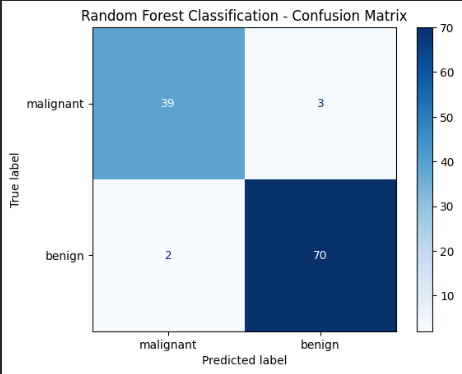
\includegraphics[width=\linewidth]{rfc_confusion_matrix.png}
    \caption{Confusion matrix}
\end{subfigure}
\hfill
\begin{subfigure}{0.48\textwidth}
    \centering
    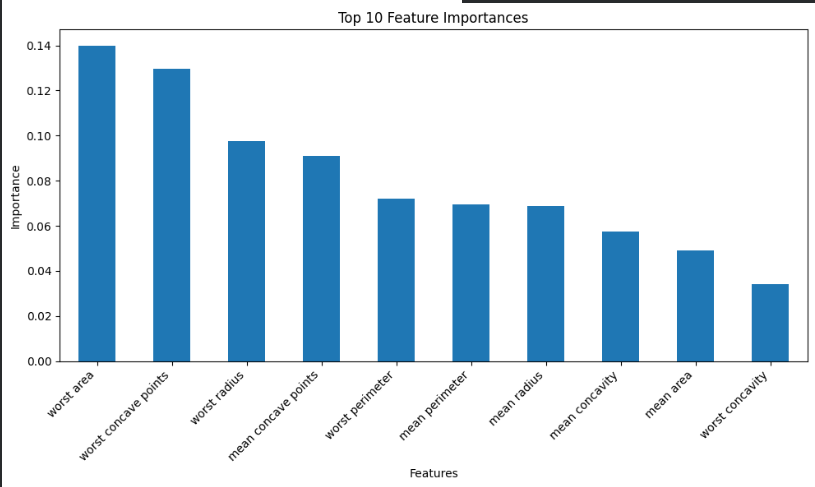
\includegraphics[width=\linewidth]{rfc_feature_importance.png}
    \caption{Top-10 feature importances}
\end{subfigure}
\caption{Random Forest classification results.}
\end{figure}

\subsubsection{Discussion \& Conclusion}
RFC achieved \(95.61\%\) accuracy with balanced precision/recall/F1 across both classes. The confusion matrix shows very few misclassifications (mainly 3 malignant samples). Feature importance ranked \emph{worst area}, \emph{worst perimeter}, and \emph{mean concave points} among the most informative features. The model needs no feature scaling and is robust, but training time grows with the number of trees and feature importance does not imply causation.

% ------------------------------------------------------------
% EXPERIMENT 10: XGBOOST
% ------------------------------------------------------------
\subsection{Experiment 10: XGBoost}

\subsubsection{Objective}
Implement XGBoost (Extreme Gradient Boosting) for classification and evaluate with Accuracy, Precision, Recall, F1, and Confusion Matrix.

\subsubsection{Dataset}
Breast Cancer Wisconsin: 569 samples, 30 features, 2 classes (malignant, benign).

\subsubsection{Theory}
XGBoost is an ensemble method based on Gradient Boosting. Trees are built \emph{sequentially}, each correcting the errors of previous trees. Regularization reduces overfitting.

\textbf{Parameters:} \texttt{n\_estimators}, \texttt{max\_depth}, \texttt{learning\_rate}, \texttt{random\_state}.

\textbf{Metrics:} Accuracy, Precision, Recall, F1, Confusion Matrix.

\textbf{vs.\ Random Forest:} RF builds trees independently (bagging + voting); XGBoost builds trees additively on residuals (boosting), often yielding higher accuracy but more tuning.

\subsubsection{Procedure}
\begin{enumerate}[nosep]
    \item Load dataset, split 80/20 (stratified).
    \item Fit \texttt{XGBClassifier(n\_estimators=100, max\_depth=3, learning\_rate=0.1)}.
    \item Predict on test set.
    \item Compute metrics, confusion matrix, and top-10 feature importances.
\end{enumerate}

\subsubsection{Code}
\begin{lstlisting}[language=Python, caption={XGBoost Classification Implementation}]
!pip install xgboost

import numpy as np
import pandas as pd
import matplotlib.pyplot as plt
from xgboost import XGBClassifier
from sklearn.datasets import load_breast_cancer
from sklearn.model_selection import train_test_split
from sklearn.metrics import (accuracy_score, classification_report,
                             confusion_matrix, ConfusionMatrixDisplay)

data = load_breast_cancer()
X, y = data.data, data.target

X_train, X_test, y_train, y_test = train_test_split(
    X, y, test_size=0.2, random_state=42, stratify=y)

model = XGBClassifier(
    n_estimators=100, max_depth=3, learning_rate=0.1,
    objective='binary:logistic', eval_metric='logloss', random_state=42)
model.fit(X_train, y_train)
y_pred = model.predict(X_test)

print("Accuracy:", accuracy_score(y_test, y_pred))
print(classification_report(y_test, y_pred, target_names=data.target_names))

ConfusionMatrixDisplay(
    confusion_matrix=confusion_matrix(y_test, y_pred),
    display_labels=data.target_names
).plot(cmap='Blues')
plt.title('XGBoost - Confusion Matrix')
plt.show()

importance = pd.Series(model.feature_importances_,
                       index=data.feature_names).sort_values(ascending=False)
plt.figure(figsize=(10,6))
importance.head(10).plot(kind='bar')
plt.title('XGBoost - Top 10 Feature Importances')
plt.xticks(rotation=45, ha='right'); plt.tight_layout()
plt.show()
\end{lstlisting}

\subsubsection{Results}
\begin{table}[H]
\centering
\caption{XGBoost Setup \& Metrics}
\begin{tabular}{ll}
\toprule
\textbf{Item} & \textbf{Value} \\
\midrule
\texttt{n\_estimators} / \texttt{max\_depth} / \texttt{learning\_rate} & 100 / 3 / 0.1 \\
Objective / Metric & \texttt{binary:logistic} / \texttt{logloss} \\
Test Size (stratified) & 0.2 \\
Random State & 42 \\
Accuracy & 0.9474 \\
Precision (Malignant / Benign) & 0.95 / 0.95 \\
Recall (Malignant / Benign) & 0.90 / 0.97 \\
F1-score (Malignant / Benign) & 0.93 / 0.96 \\
\bottomrule
\end{tabular}
\end{table}

\begin{figure}[H]
\centering
\begin{subfigure}{0.48\textwidth}
    \centering
    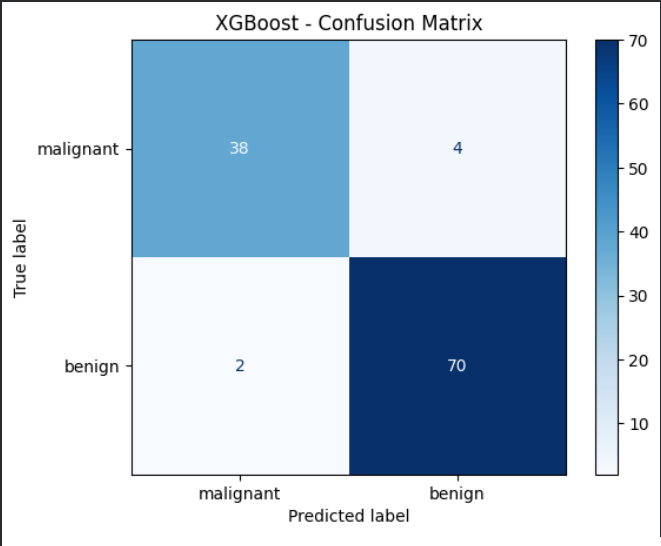
\includegraphics[width=\linewidth]{xgb_confusion_matrix.png}
    \caption{Confusion matrix}
\end{subfigure}
\hfill
\begin{subfigure}{0.48\textwidth}
    \centering
    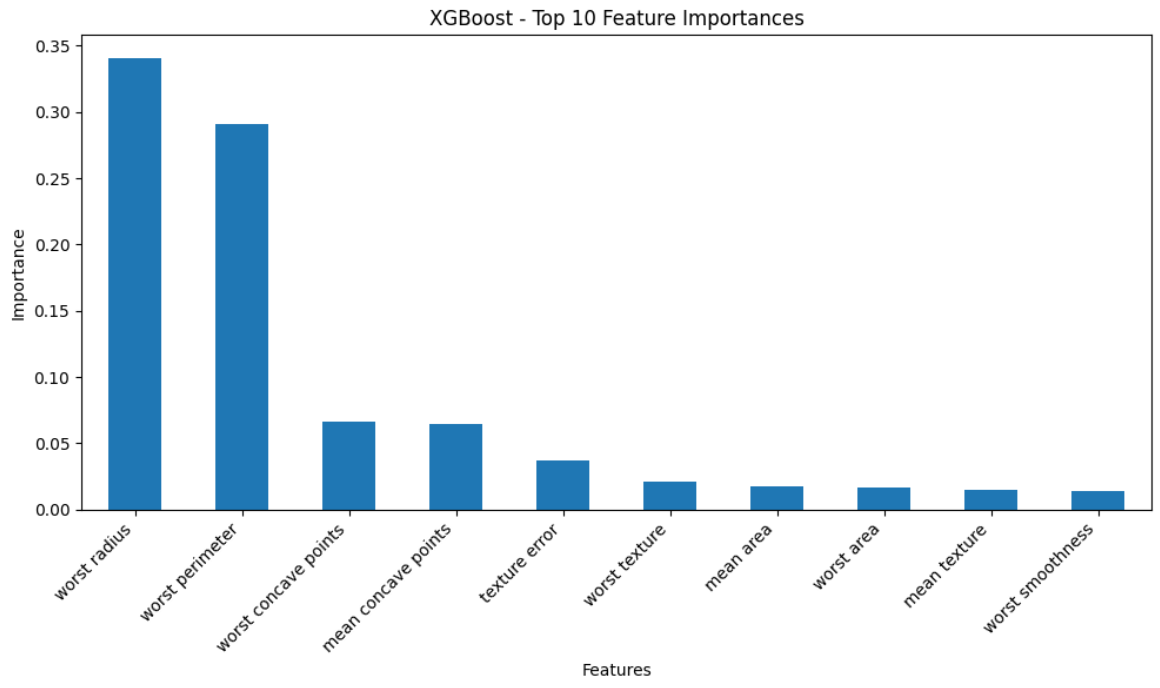
\includegraphics[width=\linewidth]{xgb_feature_importance.png}
    \caption{Top-10 feature importances}
\end{subfigure}
\caption{XGBoost classification results.}
\end{figure}

\subsubsection{Discussion \& Conclusion}
XGBoost achieved \(94.74\%\) accuracy with strong precision/recall/F1 on both classes. Misclassifications were slightly higher on the malignant class (recall \(=0.90\)) compared to benign (\(0.97\)). The sequential boosting and regularization produced performance comparable to Random Forest on this dataset. Limitations: more hyperparameters to tune, higher computational cost on large data, and risk of overfitting with poor parameter choices.

% ------------------------------------------------------------
% EXPERIMENT 11: ADABOOST
% ------------------------------------------------------------
\subsection{Experiment 11: AdaBoost}

\subsubsection{Objective}
Implement AdaBoost with Decision Stumps for classification and evaluate with Accuracy, Precision, Recall, F1, and Confusion Matrix.

\subsubsection{Dataset}
Breast Cancer Wisconsin: 569 samples, 30 features, 2 classes (malignant, benign). 80/20 stratified split.

\subsubsection{Theory}
AdaBoost (Adaptive Boosting) combines weak learners into a strong classifier. A weak learner performs slightly better than random guessing; Decision Stumps (\texttt{max\_depth=1}) are commonly used.

\textbf{Steps:}
\begin{enumerate}[nosep]
    \item Initialize equal sample weights.
    \item Train a weak learner.
    \item Increase weights of misclassified samples.
    \item Train the next learner focused on those samples.
    \item Combine learners by weighted vote.
\end{enumerate}
Sequential training makes AdaBoost sensitive to noise and outliers.

\subsubsection{Procedure}
\begin{enumerate}[nosep]
    \item Load dataset; split 80/20 (stratified).
    \item Fit \texttt{AdaBoostClassifier} with \texttt{DecisionTreeClassifier(max\_depth=1)}, \texttt{n\_estimators=50}, \texttt{learning\_rate=1.0}.
    \item Predict on test set; compute metrics and confusion matrix.
    \item Plot top-10 feature importances.
\end{enumerate}

\subsubsection{Code}
\begin{lstlisting}[language=Python, caption={AdaBoost Implementation}]
import numpy as np
import pandas as pd
import matplotlib.pyplot as plt
from sklearn.datasets import load_breast_cancer
from sklearn.model_selection import train_test_split
from sklearn.tree import DecisionTreeClassifier
from sklearn.ensemble import AdaBoostClassifier
from sklearn.metrics import (accuracy_score, classification_report,
                             confusion_matrix, ConfusionMatrixDisplay)

data = load_breast_cancer()
X, y = data.data, data.target

X_train, X_test, y_train, y_test = train_test_split(
    X, y, test_size=0.2, random_state=42, stratify=y)

base = DecisionTreeClassifier(max_depth=1, random_state=42)
model = AdaBoostClassifier(
    estimator=base, n_estimators=50, learning_rate=1.0, random_state=42)
model.fit(X_train, y_train)
y_pred = model.predict(X_test)

print("Accuracy:", accuracy_score(y_test, y_pred))
print(classification_report(y_test, y_pred, target_names=data.target_names))

ConfusionMatrixDisplay(
    confusion_matrix=confusion_matrix(y_test, y_pred),
    display_labels=data.target_names
).plot(cmap='Blues')
plt.title('AdaBoost - Confusion Matrix')
plt.show()

imp = pd.DataFrame({'Feature': data.feature_names,
                    'Importance': model.feature_importances_}
                   ).sort_values('Importance', ascending=False)

plt.figure(figsize=(10,6))
plt.barh(imp['Feature'].head(10)[::-1], imp['Importance'].head(10)[::-1])
plt.xlabel('Importance'); plt.title('Top 10 Feature Importances - AdaBoost')
plt.tight_layout(); plt.show()
\end{lstlisting}

\subsubsection{Results}
\begin{table}[H]
\centering
\caption{AdaBoost Setup \& Metrics}
\begin{tabular}{ll}
\toprule
\textbf{Item} & \textbf{Value} \\
\midrule
Base Estimator & Decision Stump (\texttt{max\_depth=1}) \\
\texttt{n\_estimators} / \texttt{learning\_rate} & 50 / 1.0 \\
Test Size (stratified) & 0.2 \\
Random State & 42 \\
Accuracy & 0.9561 \\
Precision (Malignant / Benign) & 0.97 / 0.95 \\
Recall (Malignant / Benign) & 0.90 / 0.99 \\
F1-score (Malignant / Benign) & 0.94 / 0.97 \\
\bottomrule
\end{tabular}
\end{table}

\begin{figure}[H]
\centering
\begin{subfigure}{0.48\textwidth}
    \centering
    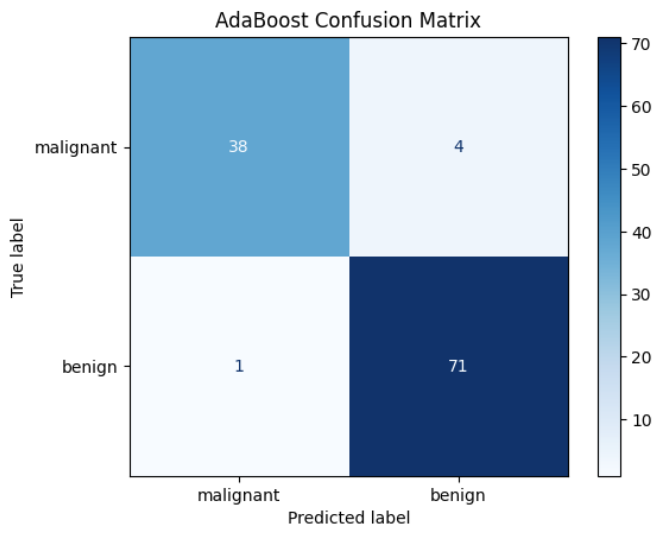
\includegraphics[width=\linewidth]{adaboost_confusion.png}
    \caption{Confusion matrix}
\end{subfigure}
\hfill
\begin{subfigure}{0.48\textwidth}
    \centering
    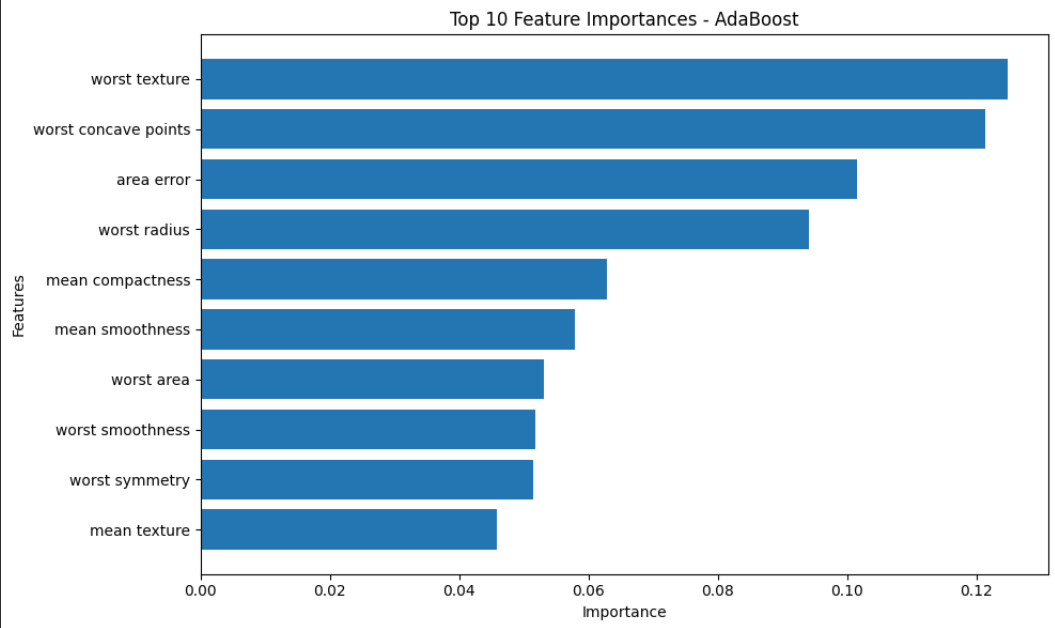
\includegraphics[width=\linewidth]{adaboost_features.png}
    \caption{Top-10 feature importances}
\end{subfigure}
\caption{AdaBoost classification results.}
\end{figure}

\subsubsection{Discussion \& Conclusion}
AdaBoost achieved \(95.61\%\) accuracy using 50 Decision Stumps. Combining weak learners into a weighted ensemble yielded performance comparable to Random Forest and XGBoost. Top features included \emph{worst texture}, \emph{worst area}, and \emph{worst perimeter}. Limitations: sensitive to noise/outliers, sequential training prevents parallelization, and performance depends on \texttt{n\_estimators} and \texttt{learning\_rate}.


% ------------------------------------------------------------
% EXPERIMENT 12: CATBOOST
% ------------------------------------------------------------
\subsection{Experiment 12: CatBoost}

\subsubsection{Objective}
Implement CatBoost for classification and evaluate with Accuracy, Precision, Recall, F1, and Confusion Matrix.

\subsubsection{Dataset}
Breast Cancer Wisconsin: 569 samples, 30 features, 2 classes (malignant, benign). 80/20 stratified split.

\subsubsection{Theory}
CatBoost (Categorical Boosting) is a gradient boosting algorithm that builds decision trees sequentially, each correcting the errors of previous trees. It handles categorical features automatically and uses \emph{ordered boosting} to reduce prediction bias.

\textbf{Parameters:} \texttt{iterations}, \texttt{learning\_rate}, \texttt{depth}, \texttt{loss\_function}, \texttt{random\_seed}.

\textbf{Metrics:} Accuracy, Precision, Recall, F1, Confusion Matrix.

\subsubsection{Procedure}
\begin{enumerate}[nosep]
    \item Load dataset; split 80/20 (stratified).
    \item Fit \texttt{CatBoostClassifier(iterations=100, learning\_rate=0.1, depth=6)}.
    \item Predict on test set; compute metrics and confusion matrix.
    \item Plot top-10 feature importances.
\end{enumerate}

\subsubsection{Code}
\begin{lstlisting}[language=Python, caption={CatBoost Implementation}]
!pip install catboost

import numpy as np
import pandas as pd
import matplotlib.pyplot as plt
from catboost import CatBoostClassifier
from sklearn.datasets import load_breast_cancer
from sklearn.model_selection import train_test_split
from sklearn.metrics import (accuracy_score, classification_report,
                             confusion_matrix, ConfusionMatrixDisplay)

data = load_breast_cancer()
X = pd.DataFrame(data.data, columns=data.feature_names)
y = data.target

X_train, X_test, y_train, y_test = train_test_split(
    X, y, test_size=0.2, random_state=42, stratify=y)

model = CatBoostClassifier(
    iterations=100, learning_rate=0.1, depth=6,
    loss_function='Logloss', random_seed=42, verbose=False)
model.fit(X_train, y_train)
y_pred = model.predict(X_test).ravel()

print("Accuracy:", accuracy_score(y_test, y_pred))
print(classification_report(y_test, y_pred, target_names=data.target_names))

ConfusionMatrixDisplay(
    confusion_matrix=confusion_matrix(y_test, y_pred),
    display_labels=data.target_names
).plot(cmap='Blues')
plt.title('CatBoost - Confusion Matrix')
plt.show()

imp = pd.DataFrame({'Feature': data.feature_names,
                    'Importance': model.feature_importances_}
                   ).sort_values('Importance', ascending=False)

plt.figure(figsize=(10,6))
plt.barh(imp['Feature'].head(10)[::-1], imp['Importance'].head(10)[::-1])
plt.xlabel('Importance'); plt.title('Top 10 Feature Importances - CatBoost')
plt.tight_layout(); plt.show()
\end{lstlisting}

\subsubsection{Results}
\begin{table}[H]
\centering
\caption{CatBoost Setup \& Metrics}
\begin{tabular}{ll}
\toprule
\textbf{Item} & \textbf{Value} \\
\midrule
\texttt{iterations} / \texttt{learning\_rate} / \texttt{depth} & 100 / 0.1 / 6 \\
Loss / Seed & Logloss / 42 \\
Test Size (stratified) & 0.2 \\
Accuracy & 0.9561 \\
Precision (Malignant / Benign) & 0.97 / 0.95 \\
Recall (Malignant / Benign) & 0.90 / 0.99 \\
F1-score (Malignant / Benign) & 0.94 / 0.97 \\
\bottomrule
\end{tabular}
\end{table}

\begin{figure}[H]
\centering
\begin{subfigure}{0.48\textwidth}
    \centering
    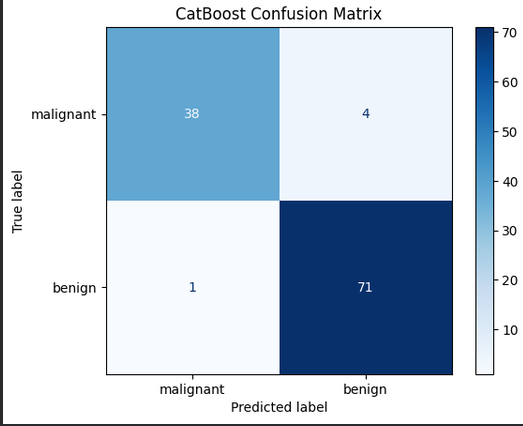
\includegraphics[width=\linewidth]{catboost_confusion.png}
    \caption{Confusion matrix}
\end{subfigure}
\hfill
\begin{subfigure}{0.48\textwidth}
    \centering
    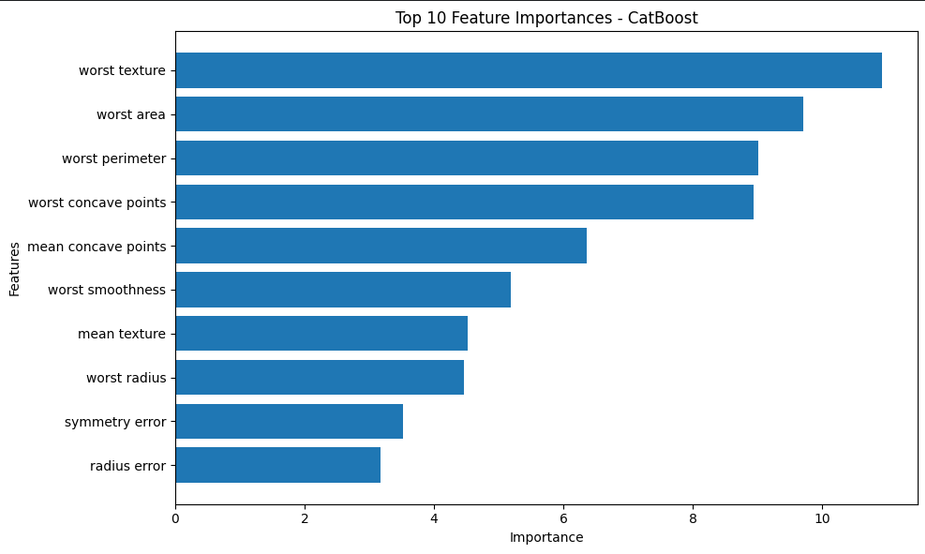
\includegraphics[width=\linewidth]{catboost_features.png}
    \caption{Top-10 feature importances}
\end{subfigure}
\caption{CatBoost classification results.}
\end{figure}

\subsubsection{Discussion \& Conclusion}
CatBoost achieved \(95.61\%\) accuracy, with strong precision/recall/F1 on both classes. Top features included \emph{worst texture}, \emph{worst area}, and \emph{worst perimeter}. Ordered boosting reduced overfitting without heavy tuning. Limitations: computationally expensive on large data, sensitive to \texttt{learning\_rate}, \texttt{depth}, and \texttt{iterations}, and this experiment uses only numerical features (categorical handling not exercised).




% ============================================================
% NEURAL LEARNING
% ============================================================
\section{Neural Learning}

% ------------------------------------------------------------
% EXPERIMENT 14: RNN
% ------------------------------------------------------------
\subsection{Experiment 14: Recurrent Neural Network (RNN)}

\subsubsection{Objective}
Implement a SimpleRNN for IMDb sentiment classification and evaluate with Accuracy, Classification Report, and Confusion Matrix.

\subsubsection{Dataset}
IMDb Movie Reviews: 25{,}000 train / 25{,}000 test, vocab \(=10{,}000\), max length \(=200\), 2 classes (positive, negative).

\subsubsection{Theory}
An RNN processes sequences step by step, maintaining a hidden state that acts as memory of past inputs. It updates the hidden state at each time step and produces an output from the final state.

Limitations: basic RNNs suffer from vanishing gradients on long sequences; LSTM/GRU handle long-range dependencies better.

\subsubsection{Procedure}
\begin{enumerate}[nosep]
    \item Load IMDb, pad sequences to length 200.
    \item Build model: Embedding (64) \(\rightarrow\) SimpleRNN (64) \(\rightarrow\) Dense (sigmoid).
    \item Train 3 epochs, batch 64, validation split 0.2.
    \item Evaluate: accuracy, classification report, confusion matrix, training curves.
\end{enumerate}

\subsubsection{Code}
\begin{lstlisting}[language=Python, caption={RNN Implementation}]
import numpy as np
import matplotlib.pyplot as plt
import tensorflow as tf
from tensorflow.keras.datasets import imdb
from tensorflow.keras.preprocessing.sequence import pad_sequences
from tensorflow.keras.models import Sequential
from tensorflow.keras.layers import Embedding, SimpleRNN, Dense
from sklearn.metrics import (accuracy_score, classification_report,
                             confusion_matrix, ConfusionMatrixDisplay)

tf.random.set_seed(42); np.random.seed(42)
vocab_size, max_length = 10000, 200

(X_train, y_train), (X_test, y_test) = imdb.load_data(num_words=vocab_size)
X_train = pad_sequences(X_train, maxlen=max_length, padding='post', truncating='post')
X_test  = pad_sequences(X_test,  maxlen=max_length, padding='post', truncating='post')

model = Sequential([
    Embedding(vocab_size, 64, input_length=max_length),
    SimpleRNN(64),
    Dense(1, activation='sigmoid')
])
model.compile(optimizer='adam', loss='binary_crossentropy', metrics=['accuracy'])

history = model.fit(X_train, y_train, epochs=3, batch_size=64,
                    validation_split=0.2, verbose=1)

loss, acc = model.evaluate(X_test, y_test, verbose=0)
y_pred = (model.predict(X_test) > 0.5).astype(int).ravel()

print("Test Loss:", loss, "| Test Accuracy:", acc)
print(classification_report(y_test, y_pred, target_names=['Negative','Positive']))

ConfusionMatrixDisplay(
    confusion_matrix=confusion_matrix(y_test, y_pred),
    display_labels=['Negative','Positive']
).plot(cmap='Blues'); plt.title('RNN Confusion Matrix'); plt.show()

plt.figure(figsize=(8,5))
plt.plot(history.history['accuracy'], label='Train')
plt.plot(history.history['val_accuracy'], label='Val')
plt.xlabel('Epoch'); plt.ylabel('Accuracy')
plt.title('RNN Accuracy'); plt.legend(); plt.grid(True); plt.show()
\end{lstlisting}

\subsubsection{Results}
\begin{table}[H]
\centering
\caption{RNN Setup \& Metrics}
\begin{tabular}{ll}
\toprule
\textbf{Item} & \textbf{Value} \\
\midrule
Vocab / Max Length / Embedding & 10{,}000 / 200 / 64 \\
RNN Units / Epochs / Batch & 64 / 3 / 64 \\
Validation Split & 0.2 \\
Test Loss & 0.7070 \\
Test Accuracy & 0.5023 \\
Precision (Neg / Pos) & 0.50 / 0.50 \\
Recall (Neg / Pos) & 0.77 / 0.23 \\
F1-score (Neg / Pos) & 0.61 / 0.32 \\
\bottomrule
\end{tabular}
\end{table}

\begin{figure}[H]
\centering
\begin{subfigure}{0.48\textwidth}
    \centering
    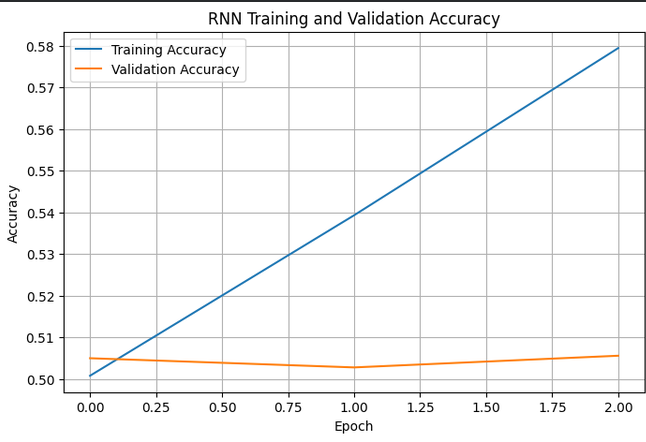
\includegraphics[width=\linewidth]{rnn_accuracy.png}
    \caption{Training/validation accuracy}
\end{subfigure}
\hfill
\begin{subfigure}{0.48\textwidth}
    \centering
    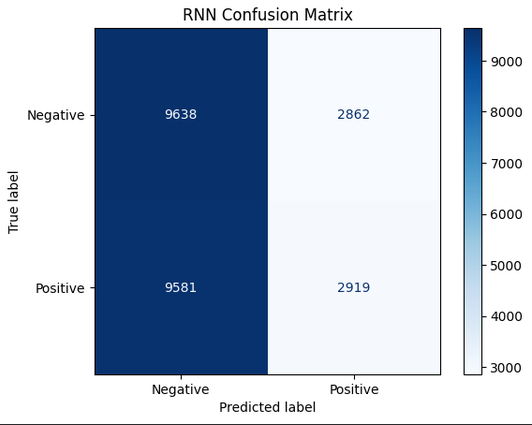
\includegraphics[width=\linewidth]{rnn_confusion.png}
    \caption{Confusion matrix}
\end{subfigure}
\caption{RNN results on IMDb.}
\end{figure}

\subsubsection{Discussion \& Conclusion}
The RNN reached only \(50.23\%\) test accuracy, close to random guessing. Recall was highly imbalanced (\(0.77\) negative vs.\ \(0.23\) positive), a sign the model collapsed to one class. Main causes: only 3 epochs, vanishing gradients across 200 timesteps, and SimpleRNN's limited capacity. LSTM/GRU or longer training would be needed for meaningful sentiment learning.

% ------------------------------------------------------------
% EXPERIMENT 15: SOM
% ------------------------------------------------------------
\subsection{Experiment 15: Self-Organizing Map (SOM)}

\subsubsection{Objective}
Implement a Self-Organizing Map (SOM) for unsupervised clustering and visualize high-dimensional Iris data on a 2D grid.

\subsubsection{Dataset}
Iris: 150 samples, 4 features, 3 classes (setosa, versicolor, virginica). Labels are used only for post-training visualization.

\subsubsection{Theory}
SOM is an unsupervised neural network that maps high-dimensional data onto a low-dimensional grid while preserving topology. It uses competitive learning:
\begin{enumerate}[nosep]
    \item Initialize neuron weights randomly.
    \item Find the Best Matching Unit (BMU) for each input.
    \item Update BMU and its neighbors toward the input.
    \item Decay learning rate and neighborhood size over iterations.
\end{enumerate}
Quantization error measures how well the map represents inputs.

\subsubsection{Procedure}
\begin{enumerate}[nosep]
    \item Standardize features.
    \item Create \(10\times10\) SOM (\texttt{sigma=1.0}, \texttt{lr=0.5}).
    \item Train 1000 iterations.
    \item Plot distance map with BMU species markers.
    \item Report quantization error and BMU coordinates.
\end{enumerate}

\subsubsection{Code}
\begin{lstlisting}[language=Python, caption={SOM Implementation}]
!pip install minisom -q

import numpy as np
import matplotlib.pyplot as plt
from minisom import MiniSom
from sklearn.datasets import load_iris
from sklearn.preprocessing import StandardScaler

iris = load_iris()
X, y = iris.data, iris.target
X_scaled = StandardScaler().fit_transform(X)

som = MiniSom(x=10, y=10, input_len=X_scaled.shape[1],
              sigma=1.0, learning_rate=0.5, random_seed=42)
som.random_weights_init(X_scaled)
som.train_random(X_scaled, num_iteration=1000)

print("Quantization Error:", som.quantization_error(X_scaled))

plt.figure(figsize=(9,7))
plt.imshow(som.distance_map(), cmap='bone_r', origin='lower')
plt.colorbar(label='Average Distance')
plt.title('SOM Distance Map')

markers = ['o','s','D']; colors = ['red','green','blue']
for i, s in enumerate(X_scaled):
    w = som.winner(s)
    plt.plot(w[0], w[1], markers[y[i]], markerfacecolor='None',
             markeredgecolor=colors[y[i]], markersize=10, markeredgewidth=2)

for i, sp in enumerate(iris.target_names):
    plt.plot([], [], markers[i], markerfacecolor='None',
             markeredgecolor=colors[i], label=sp, markersize=10, markeredgewidth=2)

plt.legend(title='Actual Species')
plt.xlabel('SOM X'); plt.ylabel('SOM Y')
plt.show()

for i in range(10):
    print(f"Sample {i+1}: {som.winner(X_scaled[i])}")
\end{lstlisting}

\subsubsection{Results}
\begin{table}[H]
\centering
\caption{SOM Setup \& Metrics}
\begin{tabular}{ll}
\toprule
\textbf{Item} & \textbf{Value} \\
\midrule
Grid & \(10\times10\) \\
Sigma / Learning Rate & 1.0 / 0.5 \\
Iterations & 1000 \\
Random Seed & 42 \\
Quantization Error & 0.2149 \\
\bottomrule
\end{tabular}
\end{table}

\begin{figure}[H]
    \centering
    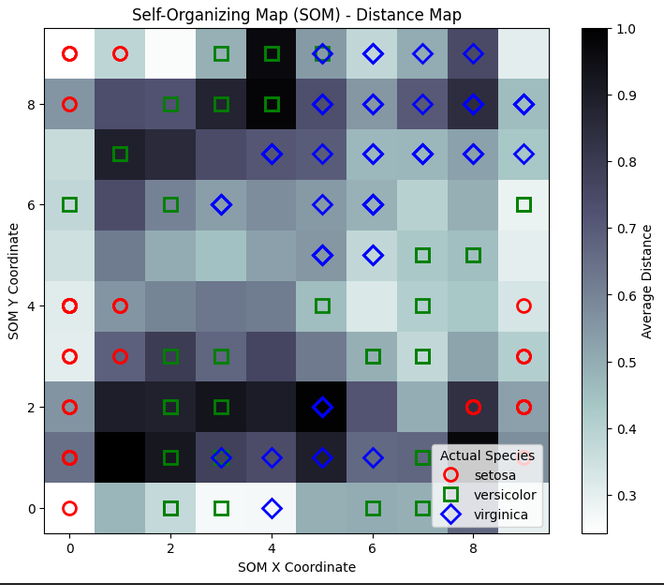
\includegraphics[width=0.8\linewidth]{som_output.png}
    \caption{SOM distance map with Iris species overlaid.}
\end{figure}

\subsubsection{Discussion \& Conclusion}
The SOM reduced 4D Iris data to a \(10\times10\) grid with quantization error \(=0.2149\). After training, species labels (not used during training) mapped to distinct regions of the grid, showing the SOM preserved topological relationships. Samples of the same species typically landed near each other (e.g., samples 2, 4, 10 clustered around \((8,2)\)--\((9,2)\)). Limitations: results depend on grid size, sigma, learning rate, and iterations; clusters must be inferred from the distance map; and results can vary across runs due to random initialization.
% ============================================================
% PROBABILISTIC LEARNING
% ============================================================
% ============================================================
% PROBABILISTIC & SEQUENCE MODELS
% ============================================================
\section{Probabilistic \& Sequence Models}

% ------------------------------------------------------------
% EXPERIMENT 16: HMM
% ------------------------------------------------------------
\subsection{Experiment 16: Hidden Markov Model (HMM)}

\subsubsection{Objective}
Implement a Gaussian HMM to model sequential data, predict hidden states via Viterbi, and evaluate with Adjusted Rand Index (ARI).

\subsubsection{Dataset}
Synthetic weather data: 300 samples, 2 hidden states, 2 observation features. True transition matrix:
\[
\begin{bmatrix} 0.90 & 0.10 \\ 0.15 & 0.85 \end{bmatrix}
\]

\subsubsection{Theory}
HMM models sequences with hidden states that emit observable outputs. Components: hidden states, observations, transition probabilities, emission probabilities, initial probabilities. The Viterbi algorithm finds the most likely state sequence.

\subsubsection{Procedure}
\begin{enumerate}[nosep]
    \item Generate synthetic hidden states and observations.
    \item Fit \texttt{GaussianHMM(n\_components=2, covariance\_type='full', n\_iter=100)}.
    \item Predict hidden states; compute ARI, log-likelihood, and learned transition matrix.
\end{enumerate}

\subsubsection{Code}
\begin{lstlisting}[language=Python, caption={HMM Implementation}]
!pip install hmmlearn -q

import numpy as np
import matplotlib.pyplot as plt
from hmmlearn.hmm import GaussianHMM
from sklearn.metrics import adjusted_rand_score

np.random.seed(42)
n_samples = 300

transition = np.array([[0.90, 0.10], [0.15, 0.85]])
means = np.array([[20, 40], [30, 75]])
covs = np.array([[[4,0],[0,25]], [[4,0],[0,25]]])

hidden = np.zeros(n_samples, dtype=int)
hidden[0] = np.random.choice([0, 1])
for i in range(1, n_samples):
    hidden[i] = np.random.choice([0, 1], p=transition[hidden[i-1]])

obs = np.array([np.random.multivariate_normal(means[s], covs[s]) for s in hidden])

model = GaussianHMM(n_components=2, covariance_type='full', n_iter=100, random_state=42)
model.fit(obs)
pred = model.predict(obs)

print("ARI:", adjusted_rand_score(hidden, pred))
print("Log Likelihood:", model.score(obs))
print("Learned Transition Matrix:\n", model.transmat_)

plt.figure(figsize=(12,6))
plt.subplot(2,1,1); plt.plot(hidden, drawstyle='steps-post'); plt.title('Actual Hidden States')
plt.subplot(2,1,2); plt.plot(pred, drawstyle='steps-post'); plt.title('Predicted Hidden States')
plt.tight_layout(); plt.show()

plt.figure(figsize=(8,5))
plt.scatter(obs[:,0], obs[:,1], c=pred, cmap='viridis', s=25)
plt.xlabel('Feature 1'); plt.ylabel('Feature 2')
plt.title('Observations Grouped by Predicted States')
plt.colorbar(label='Predicted State'); plt.show()
\end{lstlisting}

\subsubsection{Results}
\begin{table}[H]
\centering
\caption{HMM Setup \& Metrics}
\begin{tabular}{ll}
\toprule
\textbf{Item} & \textbf{Value} \\
\midrule
Components / Covariance & 2 / Full \\
Max Iterations & 100 \\
Adjusted Rand Index & 1.0 \\
Log Likelihood & \(-1687.27\) \\
\bottomrule
\end{tabular}
\end{table}

\begin{table}[H]
\centering
\caption{Learned Transition Matrix}
\begin{tabular}{lcc}
\toprule
\textbf{From $\backslash$ To} & \textbf{State 0} & \textbf{State 1} \\
\midrule
State 0 & 0.8712 & 0.1288 \\
State 1 & 0.1078 & 0.8922 \\
\bottomrule
\end{tabular}
\end{table}

\begin{figure}[H]
\centering
\begin{subfigure}{0.48\textwidth}
    \centering
    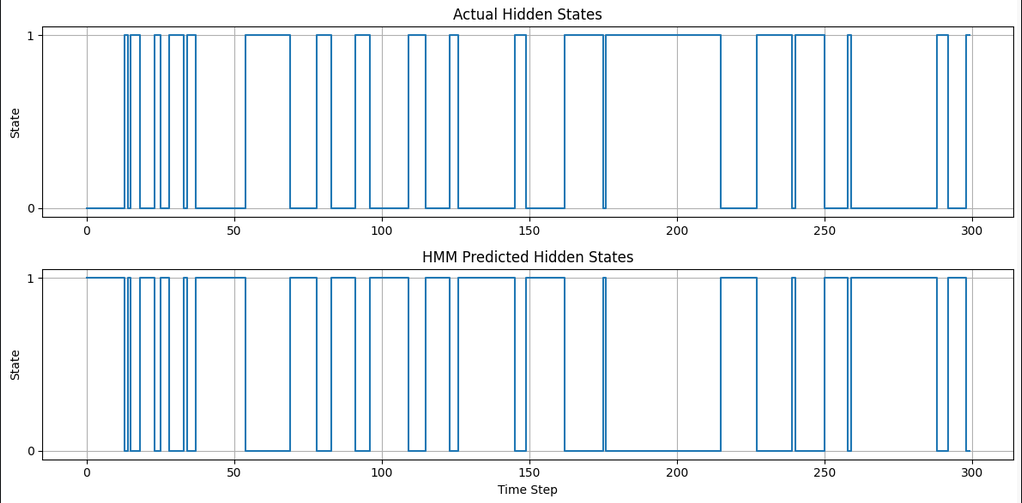
\includegraphics[width=\linewidth]{hmm_states.png}
    \caption{Actual vs.\ predicted states}
\end{subfigure}
\hfill
\begin{subfigure}{0.48\textwidth}
    \centering
    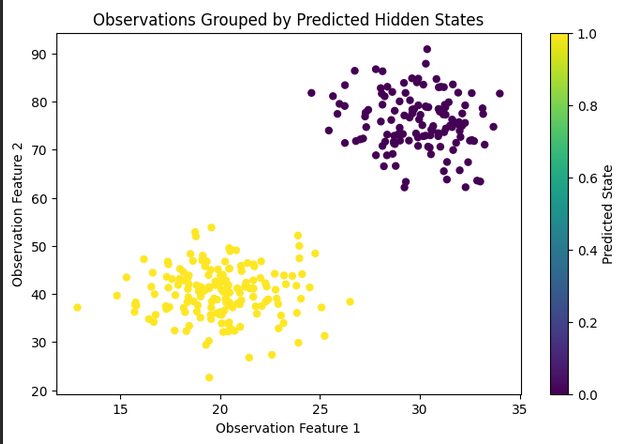
\includegraphics[width=\linewidth]{hmm_observations.png}
    \caption{Observations by predicted state}
\end{subfigure}
\caption{HMM on synthetic sequence data.}
\end{figure}

\subsubsection{Discussion \& Conclusion}
HMM achieved perfect state recovery (ARI \(=1.0\)). The learned transition matrix closely matched the true one, confirming correct identification of state persistence. Log-likelihood \(=-1687.27\) indicates a well-converged model. Limitations: Markov property may not hold in real data; number of states must be preset; emission distribution assumptions affect performance; state labels are arbitrary.



% ============================================================
% MARGIN-BASED LEARNING
% ============================================================
\section{Margin-Based Learning}

% ------------------------------------------------------------
% EXPERIMENT 17: SVM
% ------------------------------------------------------------
\subsection{Experiment 17: Support Vector Machine (SVM)}

\subsubsection{Objective}
Implement an SVM with RBF kernel for classification and evaluate with Accuracy, Precision, Recall, F1, and Confusion Matrix.

\subsubsection{Dataset}
Breast Cancer Wisconsin: 569 samples, 30 features, 2 classes (malignant, benign). 80/20 stratified split.

\subsubsection{Theory}
SVM finds the maximum-margin hyperplane separating classes. Support vectors are the closest points defining the margin. Kernels (e.g., RBF) enable non-linear boundaries. Feature scaling is essential.

\subsubsection{Procedure}
\begin{enumerate}[nosep]
    \item Load dataset, split 80/20 (stratified).
    \item Build pipeline: \texttt{StandardScaler} \(\rightarrow\) \texttt{SVC(kernel='rbf', C=1.0, gamma='scale')}.
    \item Train, predict, evaluate; report support vectors.
\end{enumerate}

\subsubsection{Code}
\begin{lstlisting}[language=Python, caption={SVM Implementation}]
import numpy as np
import matplotlib.pyplot as plt
from sklearn.datasets import load_breast_cancer
from sklearn.model_selection import train_test_split
from sklearn.preprocessing import StandardScaler
from sklearn.pipeline import Pipeline
from sklearn.svm import SVC
from sklearn.metrics import (accuracy_score, classification_report,
                             confusion_matrix, ConfusionMatrixDisplay)

data = load_breast_cancer()
X, y = data.data, data.target

X_train, X_test, y_train, y_test = train_test_split(
    X, y, test_size=0.2, random_state=42, stratify=y)

model = Pipeline([
    ('scaler', StandardScaler()),
    ('svm', SVC(kernel='rbf', C=1.0, gamma='scale'))
])
model.fit(X_train, y_train)
y_pred = model.predict(X_test)

print("Accuracy:", accuracy_score(y_test, y_pred))
print(classification_report(y_test, y_pred, target_names=data.target_names))

ConfusionMatrixDisplay(
    confusion_matrix=confusion_matrix(y_test, y_pred),
    display_labels=data.target_names
).plot(cmap='Blues')
plt.title('SVM - Confusion Matrix'); plt.show()

svm = model.named_steps['svm']
print("Support Vectors per class:", svm.n_support_)
print("Total Support Vectors:", sum(svm.n_support_))
\end{lstlisting}

\subsubsection{Results}
\begin{table}[H]
\centering
\caption{SVM Setup \& Metrics}
\begin{tabular}{ll}
\toprule
\textbf{Item} & \textbf{Value} \\
\midrule
Kernel / \(C\) / Gamma & RBF / 1.0 / scale \\
Test Size (stratified) & 0.2 \\
Accuracy & 0.9825 \\
Precision (Malignant / Benign) & 0.98 / 0.99 \\
Recall (Malignant / Benign) & 0.98 / 0.99 \\
F1-score (Malignant / Benign) & 0.98 / 0.99 \\
Support Vectors (Malignant / Benign) & 51 / 46 (total 97) \\
\bottomrule
\end{tabular}
\end{table}

\begin{figure}[H]
    \centering
    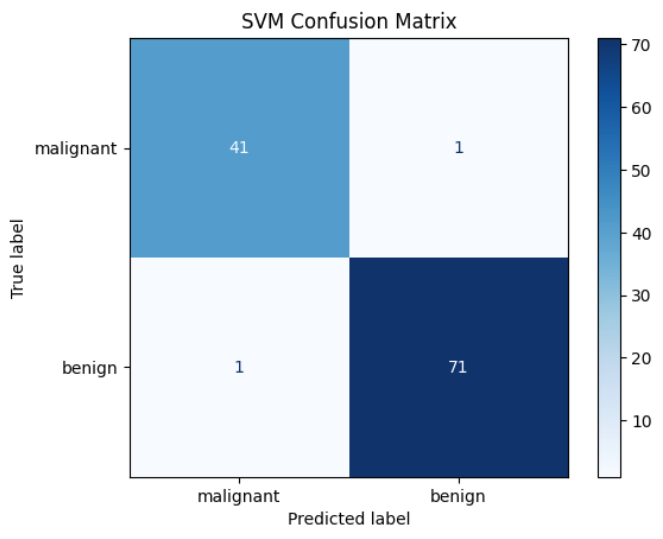
\includegraphics[width=0.7\linewidth]{svm_confusion.png}
    \caption{SVM confusion matrix.}
\end{figure}

\subsubsection{Discussion \& Conclusion}
SVM achieved \(98.25\%\) accuracy, outperforming tree-based ensembles on the same dataset. The RBF kernel captured the non-linear boundary effectively. A total of 97 support vectors out of 455 training samples indicates well-separated classes and a large margin. Limitations: slow on large datasets, sensitive to feature scaling, kernel and hyperparameter tuning required, and probability estimates are not directly available without extra cost.



% ============================================================
% GENERATIVE / FOUNDATION MODELS
% ============================================================
\section{Generative / Foundation Models}

% ------------------------------------------------------------
% EXPERIMENT 18: LLM
% ------------------------------------------------------------
\subsection{Experiment 18: Large Language Model (LLM)}

\subsubsection{Objective}
Test a pretrained LLM on multiple prompts and evaluate its responses on explanation, summarization, sentiment classification, and story generation.

\subsubsection{Setup}
Model: \texttt{google/flan-t5-small} (instruction-tuned text2text). Four user-defined prompts. Max new tokens \(=100\), greedy decoding (no sampling). Device: CPU/GPU auto-detected.

\subsubsection{Theory}
An LLM is a Transformer trained on large text corpora. Given a prompt, it tokenizes the input, predicts the next token iteratively, and generates a response. Output quality depends on model size, prompt, and generation settings. LLMs can hallucinate and should not be trusted without verification.

\subsubsection{Procedure}
\begin{enumerate}[nosep]
    \item Install \texttt{transformers} and \texttt{torch}.
    \item Load the \texttt{text2text-generation} pipeline.
    \item Feed four prompts (explain, summarize, classify, generate).
    \item Print each prompt and its generated response.
\end{enumerate}

\subsubsection{Code}
\begin{lstlisting}[language=Python, caption={LLM Prompting}]
!pip install transformers torch -q

import torch
from transformers import pipeline

device = 0 if torch.cuda.is_available() else -1
generator = pipeline('text2text-generation',
                     model='google/flan-t5-small', device=device)

prompts = [
    "Explain machine learning in simple words.",
    "Summarize this paragraph in one sentence: Artificial intelligence allows "
    "computers to perform tasks that normally require human intelligence, "
    "such as learning, reasoning, and understanding language.",
    "Classify the sentiment of this sentence as positive or negative: "
    "I really enjoyed this excellent movie.",
    "Write a short story about a student learning artificial intelligence."
]

for i, p in enumerate(prompts, 1):
    out = generator(p, max_new_tokens=100, do_sample=False)
    print(f"Experiment {i}")
    print("Prompt:", p)
    print("Response:", out[0]['generated_text'])
    print("-"*60)
\end{lstlisting}

\subsubsection{Results}
\begin{table}[H]
\centering
\caption{Prompts and Generated Responses}
\begin{tabular}{p{6cm}p{7.5cm}}
\toprule
\textbf{Prompt} & \textbf{Response} \\
\midrule
Explain ML in simple words & ``Machine learning is a process of learning.'' \\
Summarize paragraph on AI & ``Computers use artificial intelligence to perform tasks that require human intelligence.'' \\
Classify sentiment: ``I really enjoyed this excellent movie.'' & ``positive'' \\
Write a short story about a student learning AI & ``He is a student in a science class. He is a student in a science class. \dots'' (repetitive) \\
\bottomrule
\end{tabular}
\end{table}

\begin{figure}[H]
    \centering
    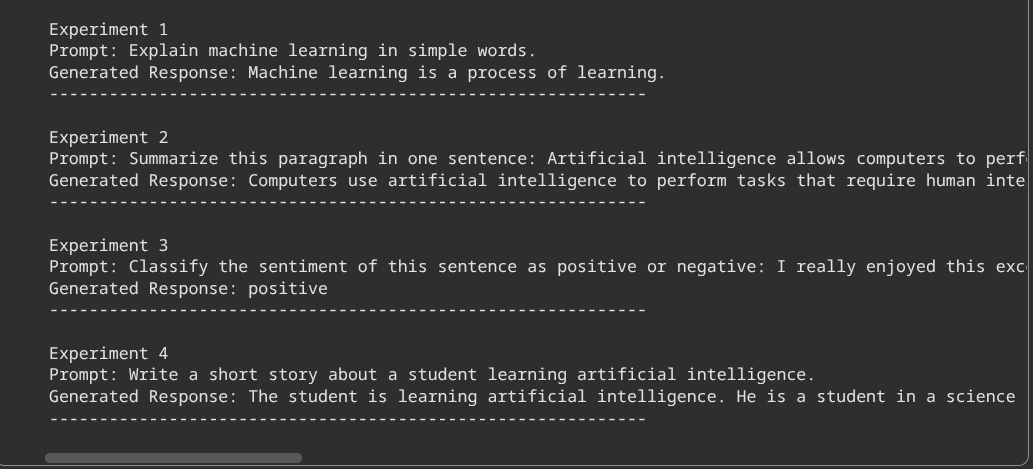
\includegraphics[width=0.85\linewidth]{llm_output.png}
    \caption{LLM output for multiple prompts.}
\end{figure}

\subsubsection{Discussion \& Conclusion}
The LLM handled short, well-defined tasks well: it correctly summarized the paragraph and classified the sentiment as ``positive.'' However, it failed on open-ended generation: the story prompt produced a repetitive loop, and the explanation was circular. These are known limits of small instruction-tuned models like FLAN-T5-small. Performance depends heavily on model size, prompt quality, and generation settings. Limitations: outputs may be incorrect or incomplete, knowledge is frozen at training cutoff, and generated responses require human verification.

% ============================================================
% ============================================================
% NON-PARAMETRIC LEARNING
% ============================================================
\section{Non-Parametric Learning}

% ------------------------------------------------------------
% EXPERIMENT 19: GRNN
% ------------------------------------------------------------
\subsection{Experiment 19: Generalized Regression Neural Network (GRNN)}

\subsubsection{Objective}
Implement a GRNN for regression and evaluate with MAE, MSE, RMSE, and R\(^2\).

\subsubsection{Dataset}
Diabetes dataset: 442 samples, 10 features, continuous target. 80/20 split, random state \(=42\).

\subsubsection{Theory}
GRNN is a non-parametric regression model that stores all training samples and predicts by similarity-based weighted averaging. Layers: input \(\rightarrow\) pattern (RBF similarity) \(\rightarrow\) summation (weighted sums) \(\rightarrow\) output.

For a new input, distances to all training samples are computed, weights are assigned by a Gaussian kernel, and the prediction is the weighted average of training targets:
\[
\hat{y} = \frac{\sum_i w_i y_i}{\sum_i w_i}, \qquad w_i = \exp\!\left(-\frac{\|x - x_i\|^2}{2\sigma^2}\right)
\]
The smoothing parameter \(\sigma\) controls the influence radius. Feature scaling is essential because GRNN uses Euclidean distances.

\subsubsection{Procedure}
\begin{enumerate}[nosep]
    \item Load dataset, split 80/20.
    \item Standardize features.
    \item Predict via Gaussian-kernel weighted average (\(\sigma=0.5\)).
    \item Compute MAE, MSE, RMSE, R\(^2\); plot actual vs.\ predicted.
\end{enumerate}

\subsubsection{Code}
\begin{lstlisting}[language=Python, caption={GRNN Implementation}]
import numpy as np
import matplotlib.pyplot as plt
from sklearn.datasets import load_diabetes
from sklearn.model_selection import train_test_split
from sklearn.preprocessing import StandardScaler
from sklearn.metrics import mean_absolute_error, mean_squared_error, r2_score

data = load_diabetes()
X, y = data.data, data.target

X_train, X_test, y_train, y_test = train_test_split(
    X, y, test_size=0.2, random_state=42)

scaler = StandardScaler()
X_train = scaler.fit_transform(X_train)
X_test  = scaler.transform(X_test)

def grnn_predict(X_train, y_train, X_test, sigma=0.5):
    preds = []
    for s in X_test:
        d = np.sum((X_train - s)**2, axis=1)
        w = np.exp(-d / (2 * sigma**2))
        preds.append(np.sum(w * y_train) / np.sum(w))
    return np.array(preds)

y_pred = grnn_predict(X_train, y_train, X_test, sigma=0.5)

mae  = mean_absolute_error(y_test, y_pred)
mse  = mean_squared_error(y_test, y_pred)
rmse = np.sqrt(mse)
r2   = r2_score(y_test, y_pred)

print("MAE:", mae, "| MSE:", mse)
print("RMSE:", rmse, "| R2:", r2)
for i in range(10):
    print(f"Actual: {y_test[i]:.2f}, Predicted: {y_pred[i]:.2f}")

plt.figure(figsize=(8,6))
plt.scatter(y_test, y_pred, alpha=0.7)
mn, mx = min(y_test.min(), y_pred.min()), max(y_test.max(), y_pred.max())
plt.plot([mn, mx], [mn, mx], 'r--', label='Perfect Prediction')
plt.xlabel('Actual'); plt.ylabel('Predicted')
plt.title('GRNN: Actual vs Predicted')
plt.legend(); plt.grid(True); plt.show()
\end{lstlisting}

\subsubsection{Results}
\begin{table}[H]
\centering
\caption{GRNN Metrics}
\begin{tabular}{ll}
\toprule
\textbf{Metric} & \textbf{Value} \\
\midrule
MAE & 42.1565 \\
MSE & 3278.28 \\
RMSE & 57.2563 \\
R\(^2\) Score & 0.3812 \\
\bottomrule
\end{tabular}
\end{table}

\begin{table}[H]
\centering
\caption{Actual vs Predicted (First 10 Samples)}
\begin{tabular}{ccc}
\toprule
\textbf{Sample} & \textbf{Actual} & \textbf{Predicted} \\
\midrule
1 & 219.00 & 216.95 \\
2 & 70.00 & 151.75 \\
3 & 202.00 & 158.29 \\
4 & 230.00 & 242.77 \\
5 & 111.00 & 113.35 \\
6 & 84.00 & 132.56 \\
7 & 242.00 & 239.14 \\
8 & 272.00 & 145.75 \\
9 & 94.00 & 103.89 \\
10 & 96.00 & 78.69 \\
\bottomrule
\end{tabular}
\end{table}

\begin{figure}[H]
    \centering
    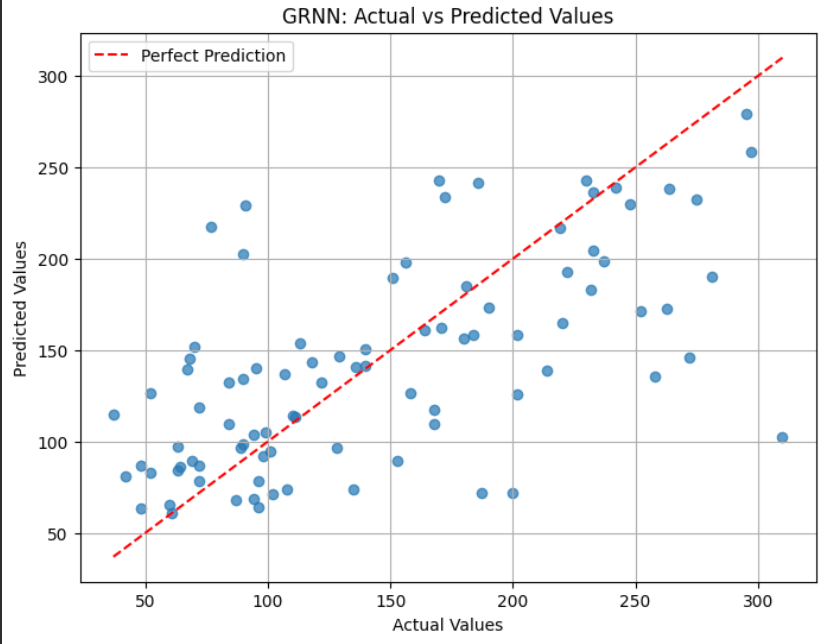
\includegraphics[width=0.7\linewidth]{grnn_output.png}
    \caption{GRNN: actual vs.\ predicted values.}
\end{figure}

\subsubsection{Discussion \& Conclusion}
GRNN achieved R\(^2=0.3812\), RMSE \(=57.26\), and MAE \(=42.16\), explaining about \(38\%\) of the target variance. The model predicted mid-range values well (e.g., sample 1: \(219\) vs.\ \(216.95\)) but under-fit extremes (sample 8: \(272\) vs.\ \(145.75\)), a known effect of weighted averaging. Performance is highly sensitive to \(\sigma\): smaller values overfit, larger values oversmooth. Cross-validation to tune \(\sigma\) would likely improve R\(^2\). Limitations: stores all training samples (high memory), slow prediction for large datasets, requires feature scaling, and tends to under-predict extreme targets.

\end{document}